\documentclass[aspectratio=169,10pt]{beamer}
\usetheme{metropolis}
\usecolortheme{default}

% Color definitions
\definecolor{primaryblue}{RGB}{20,75,140}
\definecolor{secondaryblue}{RGB}{70,130,180}
\definecolor{accentorange}{RGB}{230,95,45}

% Set theme colors
\setbeamercolor{title}{fg=primaryblue}
\setbeamercolor{frametitle}{fg=primaryblue}
\setbeamercolor{progress bar}{fg=accentorange, bg=primaryblue}
\setbeamercolor{alerted text}{fg=accentorange}

% Math packages
\usepackage{amsmath}
\usepackage{amsfonts}
\usepackage{amssymb}
\usepackage{bm}

% Graphics and tables
\usepackage{graphicx}
\usepackage{booktabs}
\usepackage{array}
\usepackage{tikz}

% Custom alert boxes
\usepackage{tcolorbox}
\tcbuselibrary{theorems}

\newtcbtheorem[number within=section]{keypoint}{Key Point}%
{colback=primaryblue!5,colframe=primaryblue,fonttitle=\bfseries,
 arc=2mm,boxrule=1pt}{kp}

\newtcbtheorem[number within=section]{insight}{Insight}%
{colback=accentorange!5,colframe=accentorange,fonttitle=\bfseries,
 arc=2mm,boxrule=1pt}{in}

% Title information
\title{Image Restoration and Geometric Processing}
\subtitle{CMSC 178IP - Digital Image Processing}
\author{Noel Jeffrey Pinton}
\institute{University of the Philippines - Cebu\\Department of Computer Science}
\date{} % Leave empty - no date on title slide

\begin{document}

% Title slide
\begin{frame}
    \titlepage
\end{frame}

% Table of contents
\begin{frame}{Outline}
    \tableofcontents
\end{frame}

\section{Introduction to Image Restoration}

\begin{frame}{What is Image Restoration?}
    \begin{columns}[T]
        \begin{column}{0.6\textwidth}
            \textbf{Image Restoration} is the process of recovering an original image from a degraded version.

            \vspace{0.5cm}
            \textbf{Key Characteristics:}
            \begin{itemize}
                \item Objective process with known degradation model
                \item Attempts to reverse known distortions
                \item Uses mathematical and probabilistic models
                \item Quality can be measured quantitatively
            \end{itemize}
        \end{column}
        \begin{column}{0.35\textwidth}
            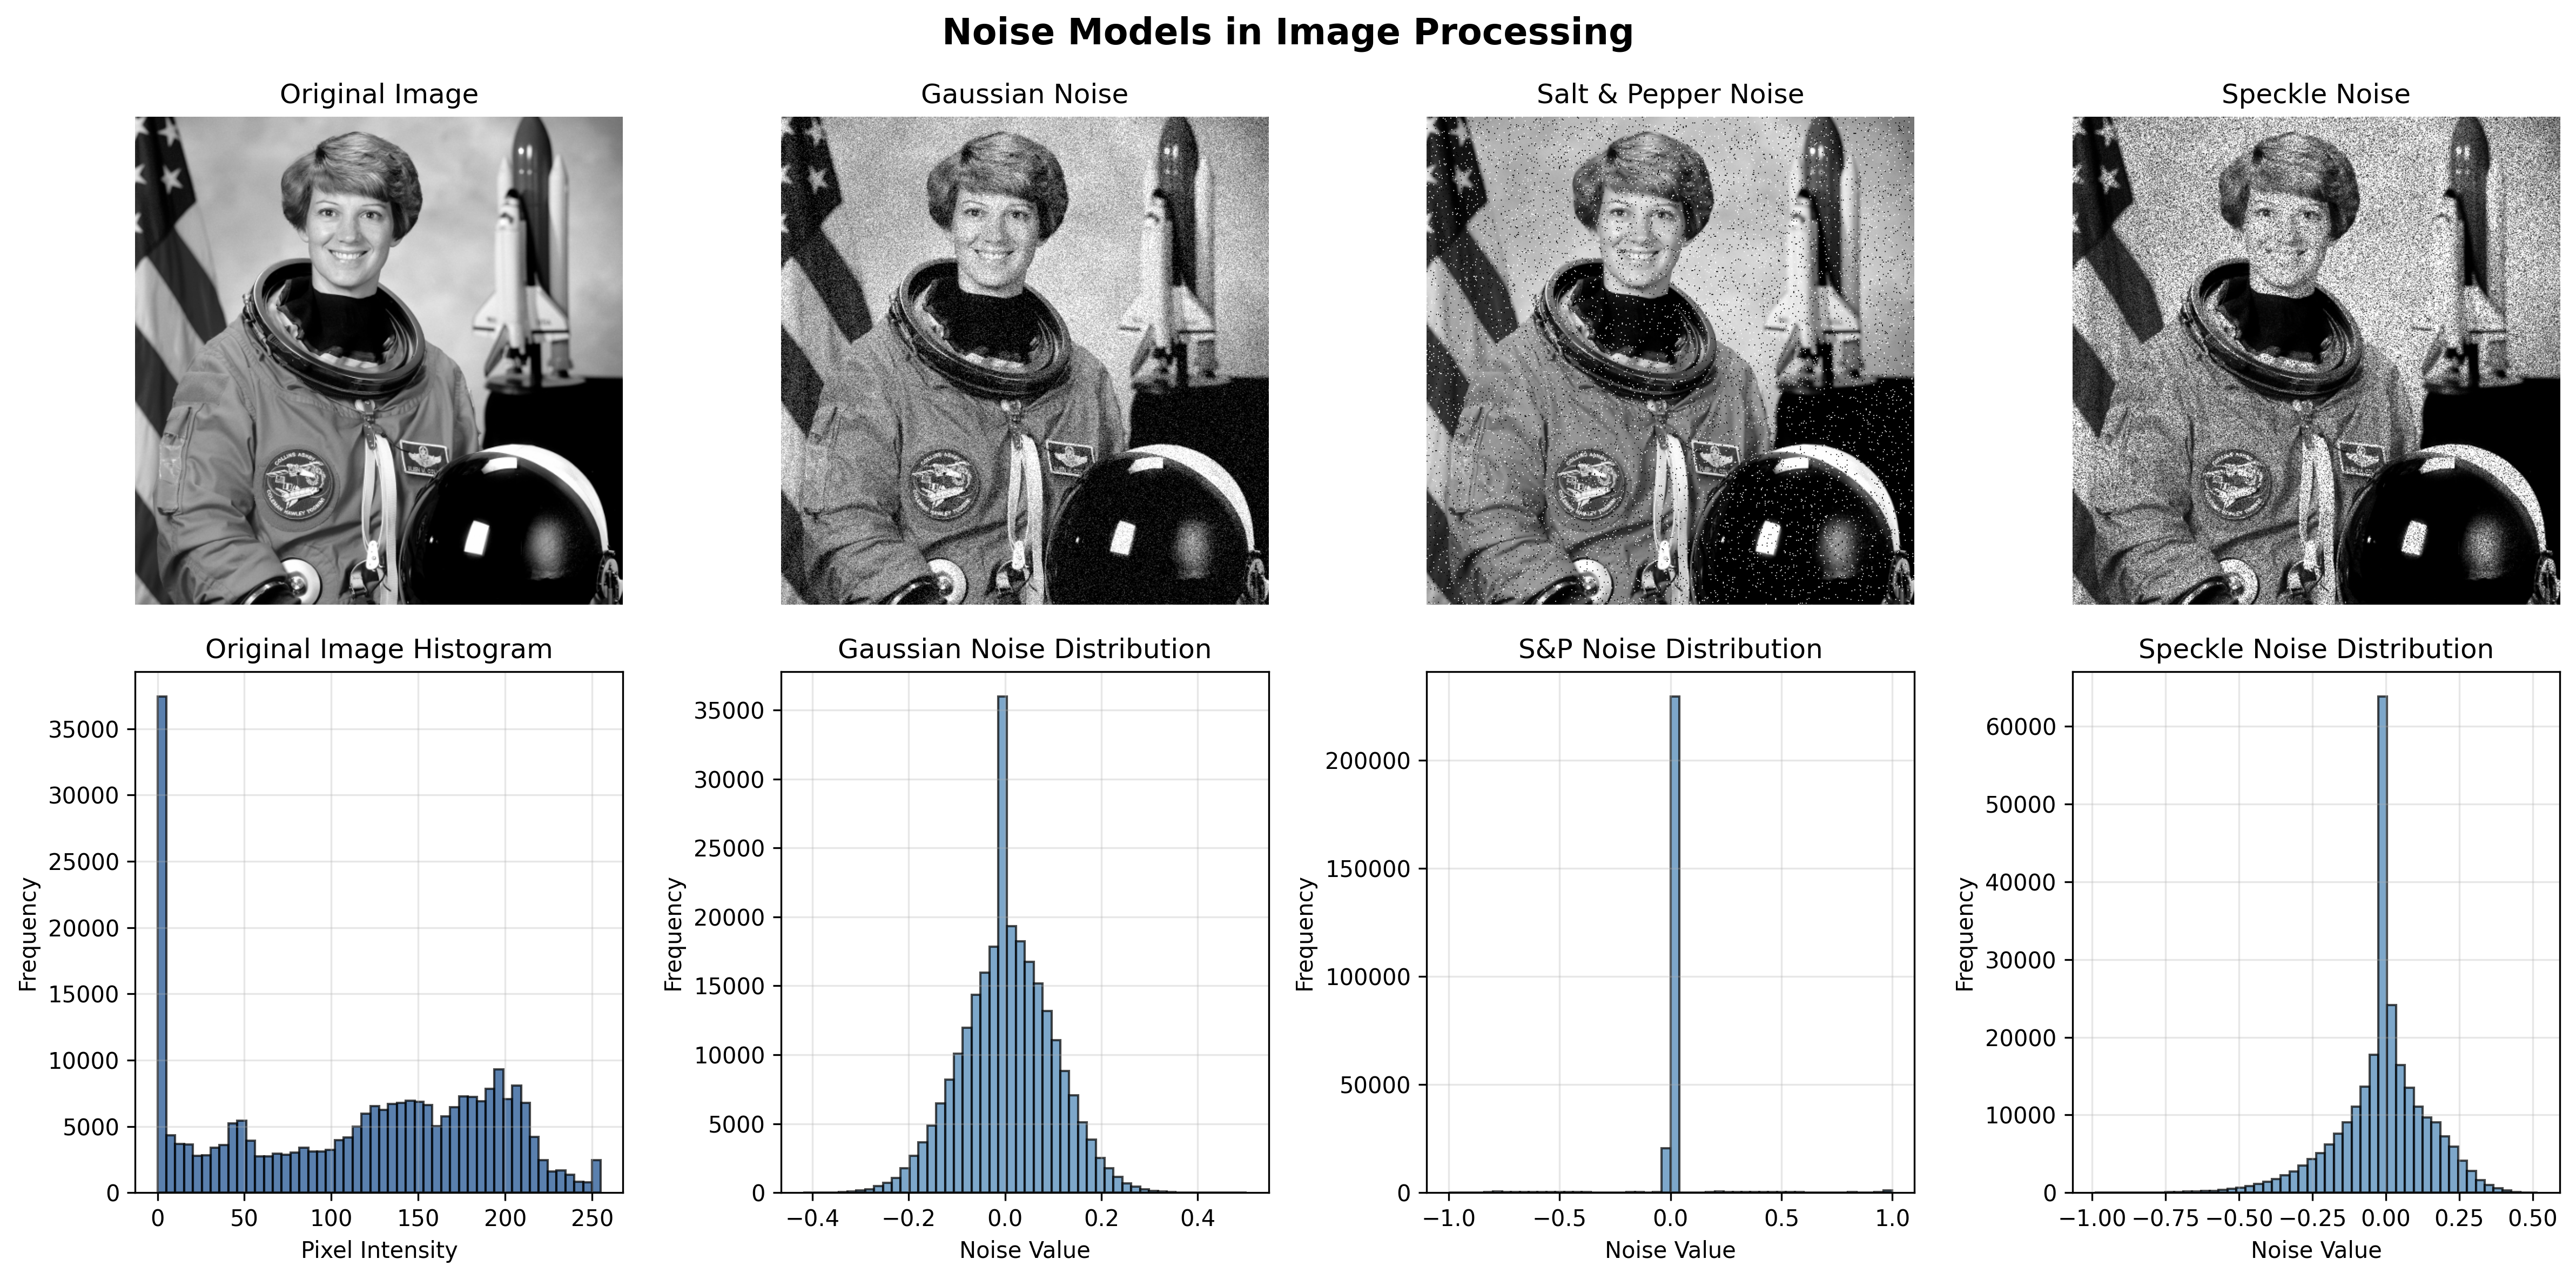
\includegraphics[width=\textwidth]{../figures/noise_models.png}
        \end{column}
    \end{columns}

    \begin{keypoint}{Restoration vs Enhancement}{}
        \textbf{Restoration:} Recovers image based on degradation model\\
        \textbf{Enhancement:} Improves visual appearance subjectively
    \end{keypoint}
\end{frame}

\begin{frame}{Image Degradation Model}
    \begin{columns}[T]
        \begin{column}{0.6\textwidth}
            The fundamental degradation model:
            \begin{equation}
                g(x,y) = h(x,y) * f(x,y) + \eta(x,y)
            \end{equation}

            Where:
            \begin{itemize}
                \item $f(x,y)$ = original image
                \item $h(x,y)$ = degradation function (PSF)
                \item $\eta(x,y)$ = additive noise
                \item $g(x,y)$ = degraded image
                \item $*$ = convolution operator
            \end{itemize}
        \end{column}
        \begin{column}{0.35\textwidth}
            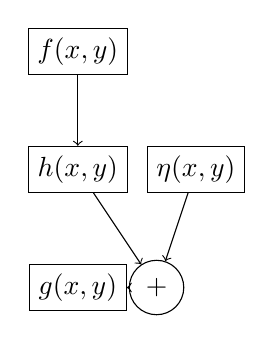
\begin{tikzpicture}[node distance=1.5cm]
                \node (input) [draw, rectangle] {$f(x,y)$};
                \node (system) [draw, rectangle, below of=input] {$h(x,y)$};
                \node (noise) [draw, rectangle, right of=system] {$\eta(x,y)$};
                \node (output) [draw, rectangle, below of=system] {$g(x,y)$};
                \node (plus) [draw, circle, right of=output, xshift=-0.5cm] {$+$};

                \draw [->] (input) -- (system);
                \draw [->] (system) -- (plus);
                \draw [->] (noise) -- (plus);
                \draw [->] (plus) -- (output);
            \end{tikzpicture}
        \end{column}
    \end{columns}
\end{frame}

\begin{frame}{Types of Image Degradation}
    \begin{columns}[T]
        \begin{column}{0.5\textwidth}
            \textbf{Common Degradation Sources:}
            \begin{itemize}
                \item \textbf{Blur:} Motion, defocus, atmospheric
                \item \textbf{Noise:} Gaussian, salt \& pepper, speckle
                \item \textbf{Geometric:} Rotation, scaling, warping
                \item \textbf{Radiometric:} Illumination changes
            \end{itemize}

            \vspace{0.3cm}
            \textbf{Noise Models:}
            \begin{itemize}
                \item Gaussian: $\eta \sim \mathcal{N}(0, \sigma^2)$
                \item Uniform: $\eta \sim U[a, b]$
                \item Salt \& Pepper: Impulse noise
            \end{itemize}
        \end{column}
        \begin{column}{0.45\textwidth}
            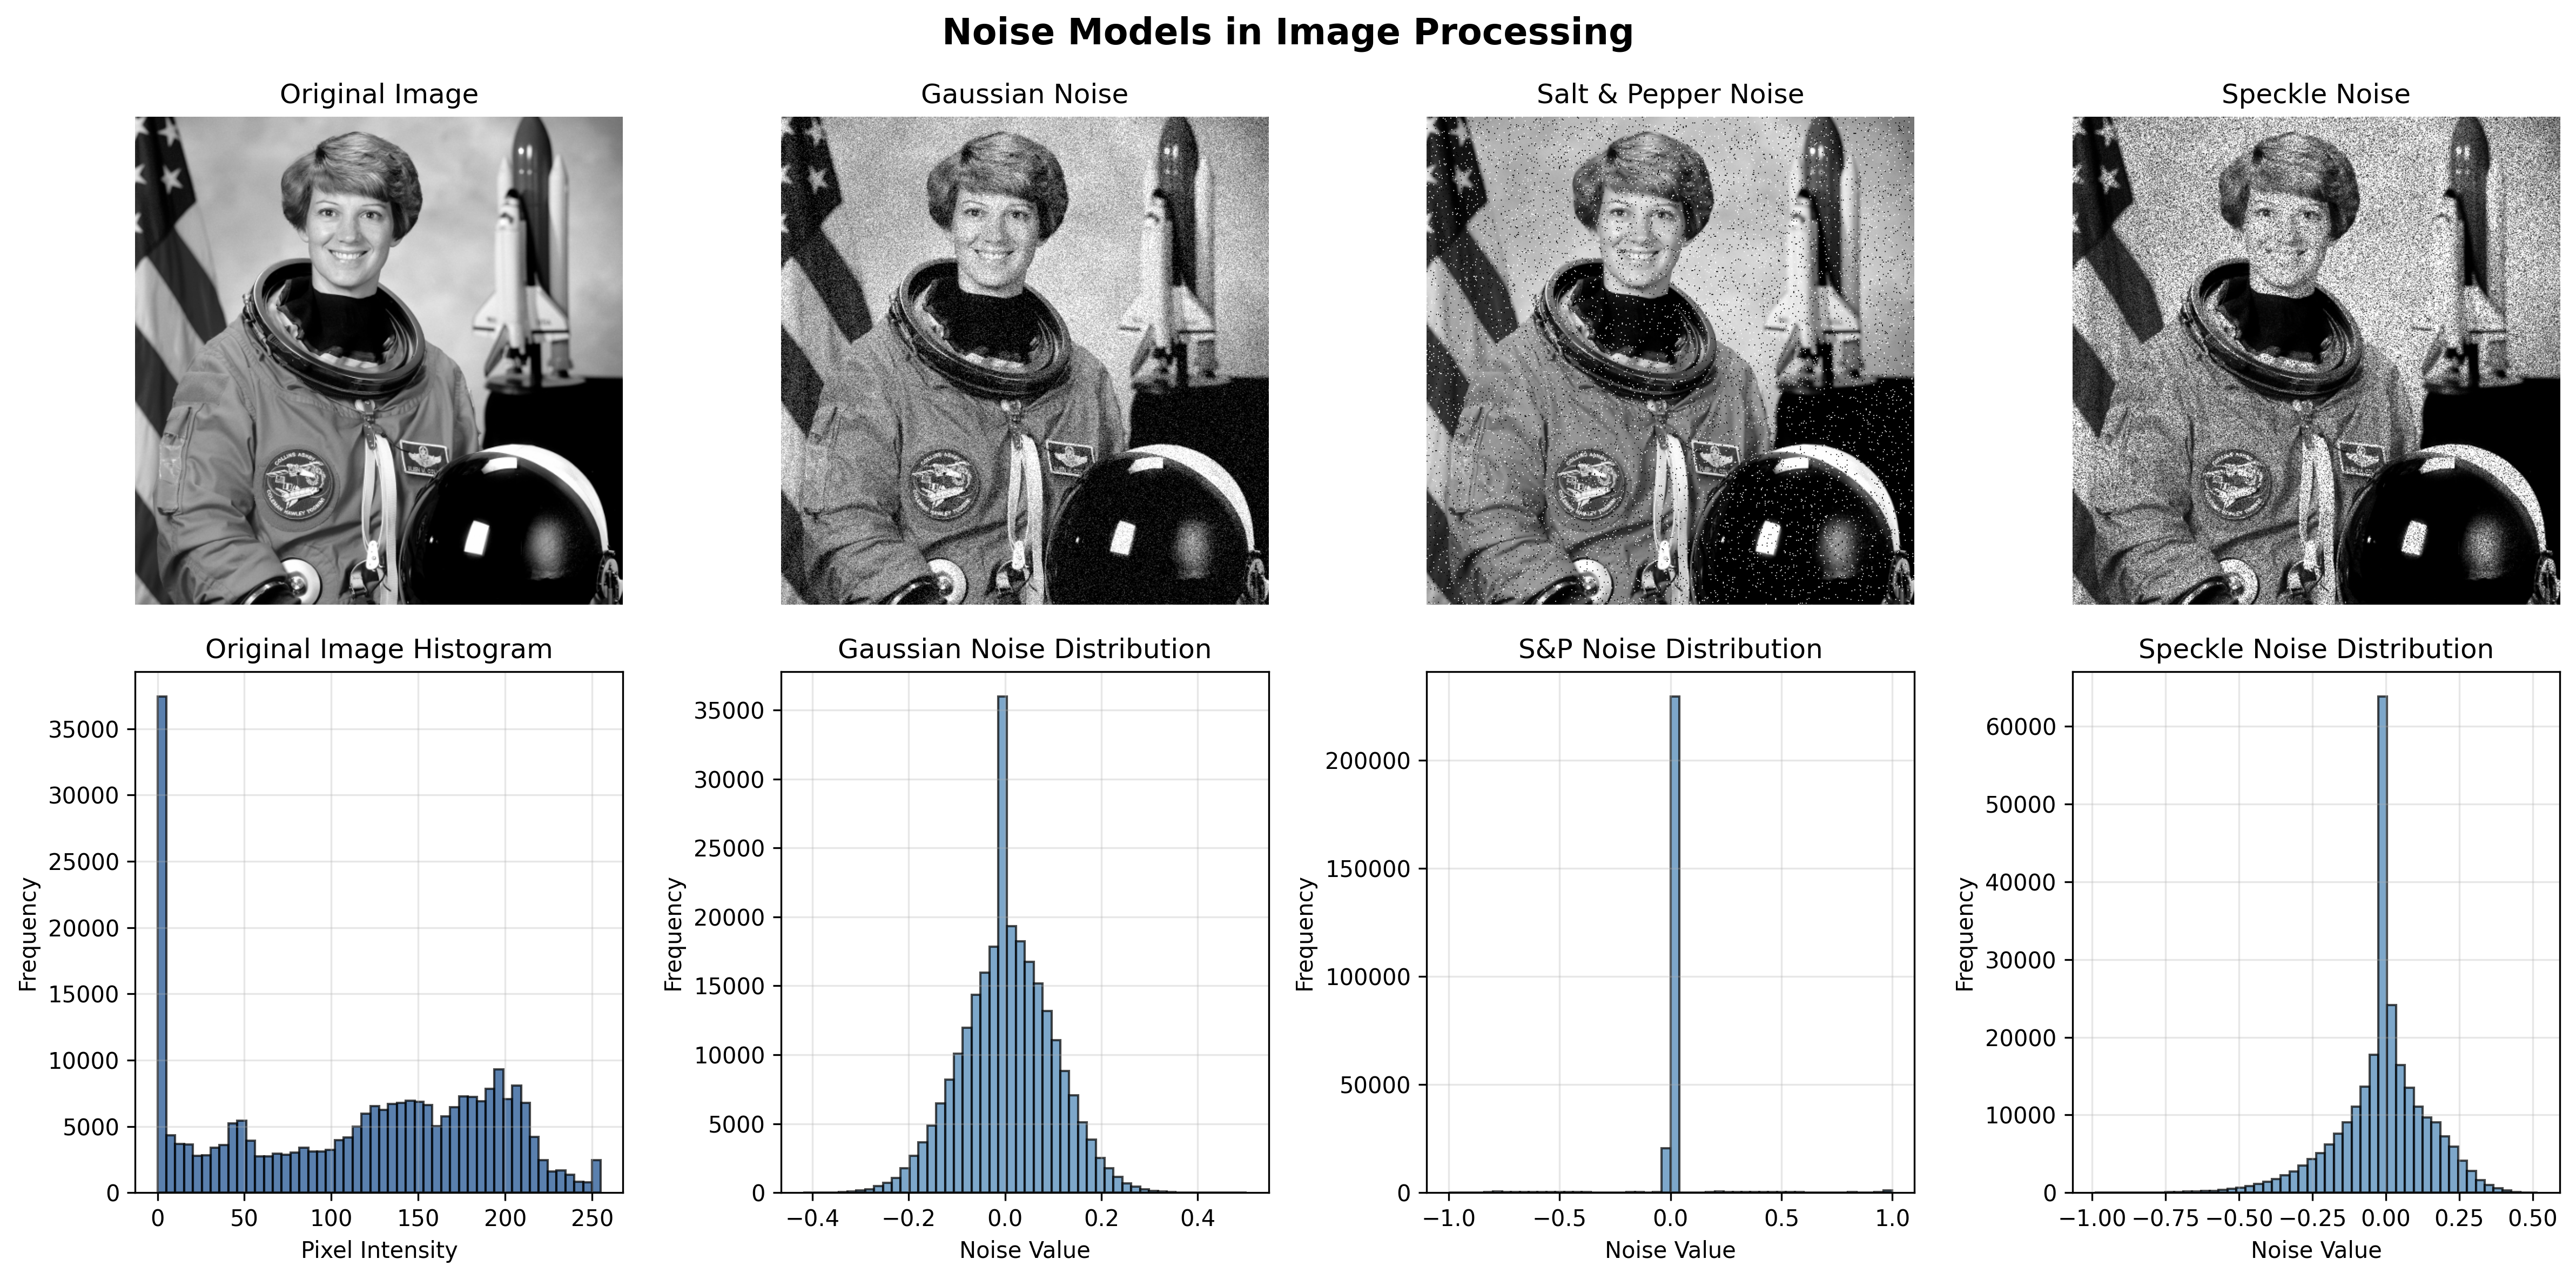
\includegraphics[width=\textwidth]{../figures/noise_models.png}
        \end{column}
    \end{columns}
\end{frame}

\section{Spatial Domain Restoration}

\begin{frame}{Spatial Filtering Techniques}
    \begin{columns}[T]
        \begin{column}{0.6\textwidth}
            \textbf{Linear Spatial Filters:}
            \begin{itemize}
                \item Mean filter: $\bar{f}(x,y) = \frac{1}{mn}\sum_{(s,t) \in S} g(s,t)$
                \item Gaussian filter: $h(x,y) = \frac{1}{2\pi\sigma^2}e^{-\frac{x^2+y^2}{2\sigma^2}}$
                \item Wiener filter: Optimal MSE restoration
            \end{itemize}

            \vspace{0.3cm}
            \textbf{Nonlinear Spatial Filters:}
            \begin{itemize}
                \item Median filter: $\tilde{f}(x,y) = \text{median}_{(s,t) \in S}\{g(s,t)\}$
                \item Bilateral filter: Edge-preserving smoothing
                \item Morphological filters
            \end{itemize}
        \end{column}
        \begin{column}{0.35\textwidth}
            
\includegraphics[width=\textwidth]{../figures/spatial_filtering.png}
        \end{column}
    \end{columns}
\end{frame}

\begin{frame}{Mean and Gaussian Filtering}
    \begin{columns}[T]
        \begin{column}{0.6\textwidth}
            \textbf{Mean Filter:}
            $$h_{mean} = \frac{1}{9}\begin{bmatrix}
            1 & 1 & 1 \\
            1 & 1 & 1 \\
            1 & 1 & 1
            \end{bmatrix}$$

            \textbf{Gaussian Filter:}
            $$h_{gauss}(x,y) = \frac{1}{2\pi\sigma^2}\exp\left(-\frac{x^2+y^2}{2\sigma^2}\right)$$

            \textbf{Properties:}
            \begin{itemize}
                \item Mean: Simple, fast, causes blurring
                \item Gaussian: Smooth, preserves edges better
            \end{itemize}
        \end{column}
        \begin{column}{0.35\textwidth}
            \begin{insight}{Filter Selection}{}
                Choose filter based on noise type and edge preservation requirements
            \end{insight}
        \end{column}
    \end{columns}
\end{frame}

\begin{frame}{Median and Bilateral Filtering}
    \begin{columns}[T]
        \begin{column}{0.6\textwidth}
            \textbf{Median Filter:}
            \begin{itemize}
                \item Excellent for salt \& pepper noise
                \item Preserves edges and fine details
                \item Nonlinear operation
            \end{itemize}

            \textbf{Bilateral Filter:}
            $$I^{bf}(x) = \frac{1}{W_p}\sum_{x_i \in \Omega} I(x_i) f_r(||I(x_i) - I(x)||) g_s(||x_i - x||)$$

            Where:
            \begin{itemize}
                \item $f_r$ = range kernel (intensity similarity)
                \item $g_s$ = spatial kernel (geometric closeness)
                \item $W_p$ = normalization factor
            \end{itemize}
        \end{column}
        \begin{column}{0.35\textwidth}
            
\includegraphics[width=\textwidth]{../figures/spatial_filtering.png}
        \end{column}
    \end{columns}
\end{frame}

\section{Frequency Domain Restoration}

\begin{frame}{Frequency Domain Approach}
    \begin{columns}[T]
        \begin{column}{0.6\textwidth}
            \textbf{Convolution Theorem:}
            $$g(x,y) = h(x,y) * f(x,y)$$
            $$\Updownarrow$$
            $$G(u,v) = H(u,v) \cdot F(u,v)$$

            \textbf{Restoration Process:}
            \begin{enumerate}
                \item Transform to frequency domain
                \item Apply restoration filter
                \item Transform back to spatial domain
            \end{enumerate}

            \textbf{Ideal Inverse Filter:}
            $$\hat{F}(u,v) = \frac{G(u,v)}{H(u,v)}$$
        \end{column}
        \begin{column}{0.35\textwidth}
            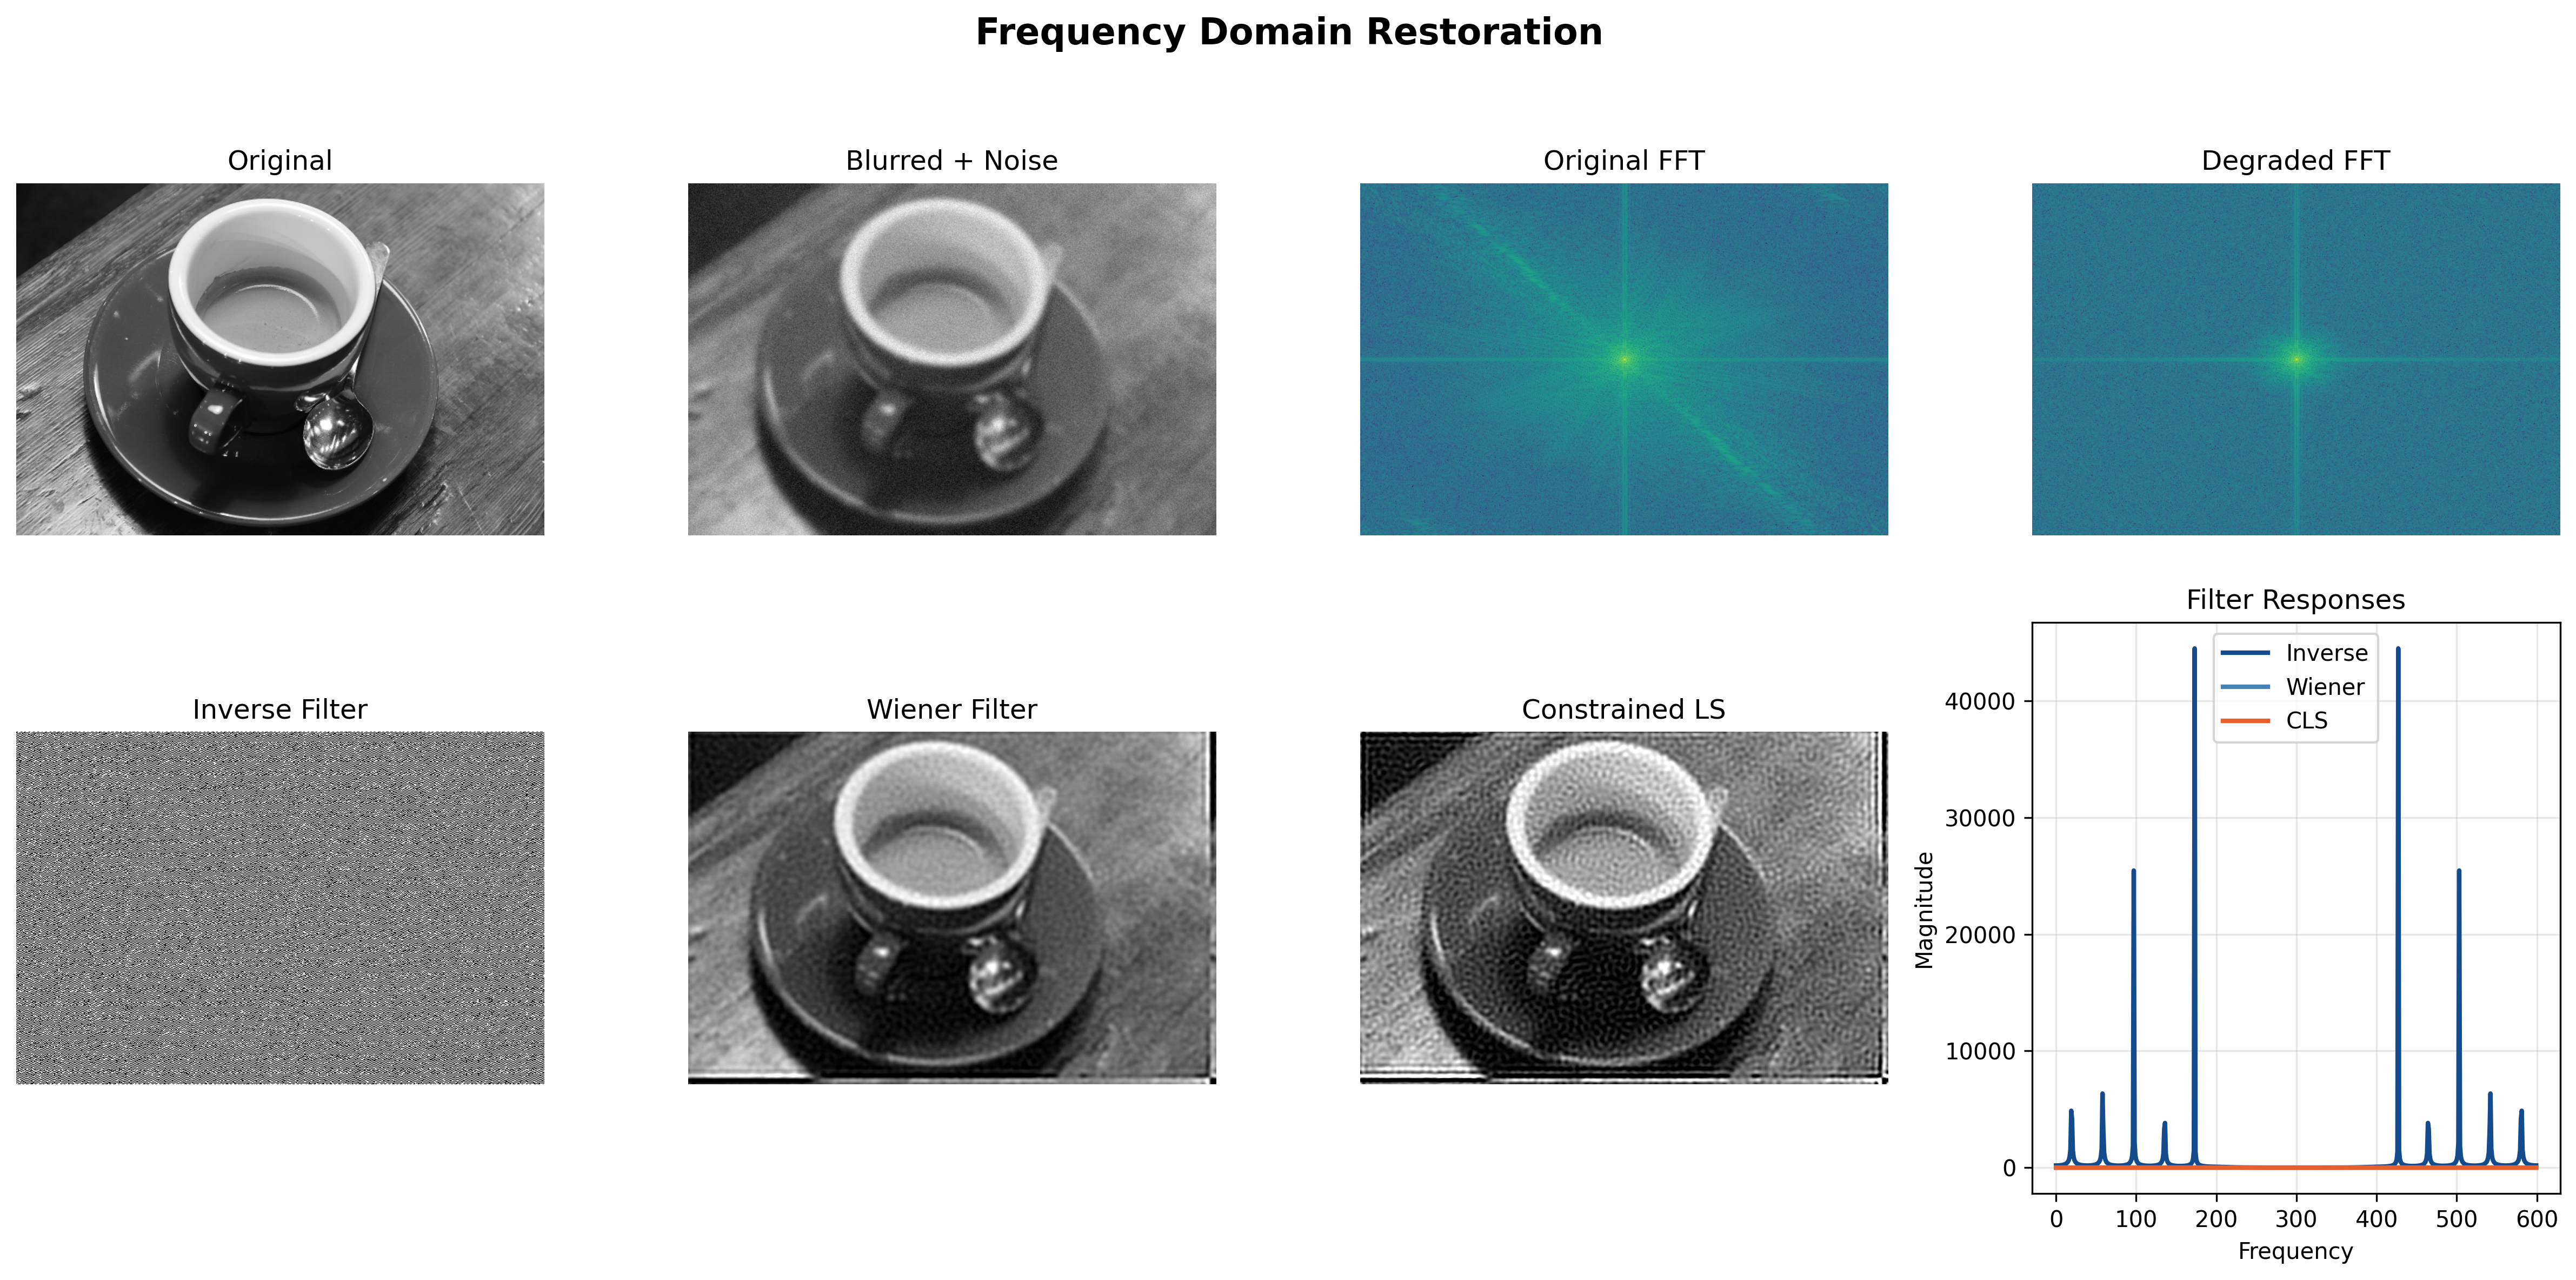
\includegraphics[width=\textwidth]{../figures/frequency_domain_restoration.png}
        \end{column}
    \end{columns}
\end{frame}

\begin{frame}{Wiener Filtering}
    \begin{columns}[T]
        \begin{column}{0.6\textwidth}
            \textbf{Wiener Filter:}
            $$H_w(u,v) = \frac{H^*(u,v)}{|H(u,v)|^2 + \frac{S_\eta(u,v)}{S_f(u,v)}}$$

            Where:
            \begin{itemize}
                \item $H^*(u,v)$ = complex conjugate of $H(u,v)$
                \item $S_\eta(u,v)$ = noise power spectrum
                \item $S_f(u,v)$ = signal power spectrum
            \end{itemize}

            \textbf{Practical Form:}
            $$H_w(u,v) = \frac{H^*(u,v)}{|H(u,v)|^2 + K}$$

            Where $K$ is the noise-to-signal power ratio.
        \end{column}
        \begin{column}{0.35\textwidth}
            \begin{keypoint}{Wiener Optimality}{}
                Minimizes mean square error between original and restored image
            \end{keypoint}
        \end{column}
    \end{columns}
\end{frame}

\begin{frame}{Constrained Least Squares Filtering}
    \begin{columns}[T]
        \begin{column}{0.6\textwidth}
            \textbf{CLS Filter:}
            $$H_{cls}(u,v) = \frac{H^*(u,v)}{|H(u,v)|^2 + \gamma|P(u,v)|^2}$$

            Where:
            \begin{itemize}
                \item $P(u,v)$ = Fourier transform of Laplacian operator
                \item $\gamma$ = regularization parameter
            \end{itemize}

            \textbf{Laplacian Operator:}
            $$p = \begin{bmatrix}
            0 & -1 & 0 \\
            -1 & 4 & -1 \\
            0 & -1 & 0
            \end{bmatrix}$$

            \textbf{Advantages:}
            \begin{itemize}
                \item No noise power spectrum needed
                \item Smoothness constraint via Laplacian
            \end{itemize}
        \end{column}
        \begin{column}{0.35\textwidth}
            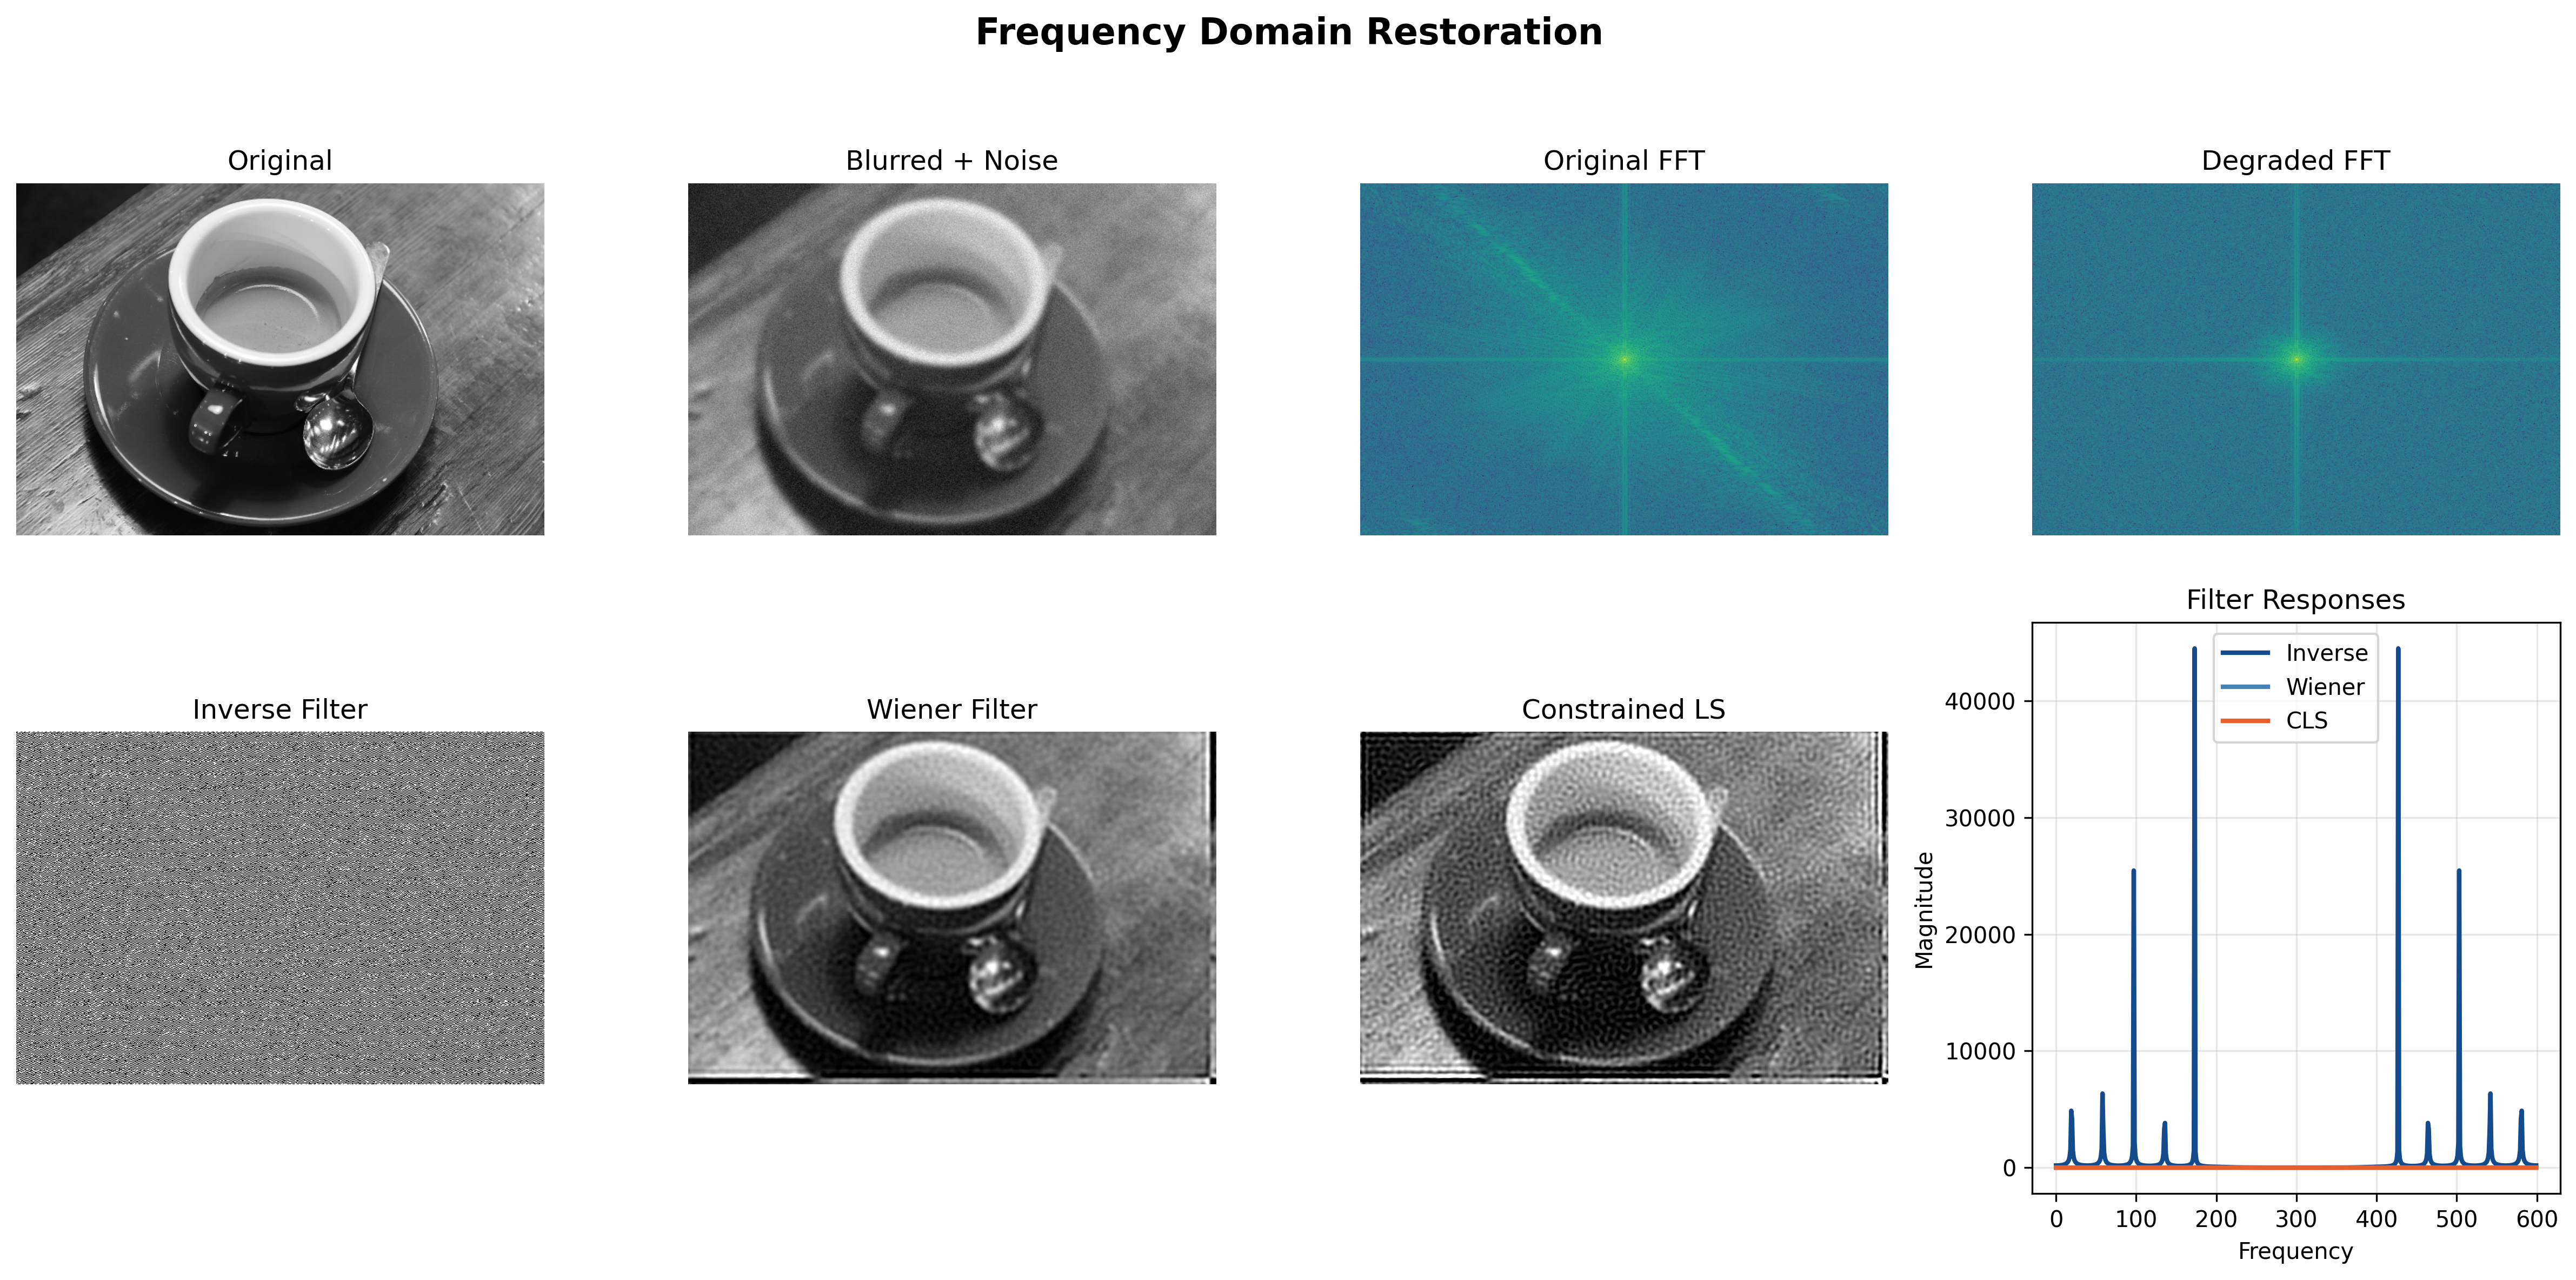
\includegraphics[width=\textwidth]{../figures/frequency_domain_restoration.png}
        \end{column}
    \end{columns}
\end{frame}

\section{Motion Blur and Deblurring}

\begin{frame}{Motion Blur Modeling}
    \begin{columns}[T]
        \begin{column}{0.6\textwidth}
            \textbf{Linear Motion Blur:}
            For motion with displacement $(a, b)$ over time $T$:

            $$H(u,v) = \frac{T}{\pi(ua+vb)} \sin[\pi(ua+vb)] e^{-j\pi(ua+vb)}$$

            \textbf{Simplified for horizontal motion:}
            $$H(u,v) = \frac{\sin(\pi ua)}{\pi ua} e^{-j\pi ua}$$

            \textbf{Motion Blur Kernel:}
            $$h(x,y) = \begin{cases}
            \frac{1}{a} & \text{if } |x| \leq \frac{a}{2}, y = 0 \\
            0 & \text{otherwise}
            \end{cases}$$
        \end{column}
        \begin{column}{0.35\textwidth}
            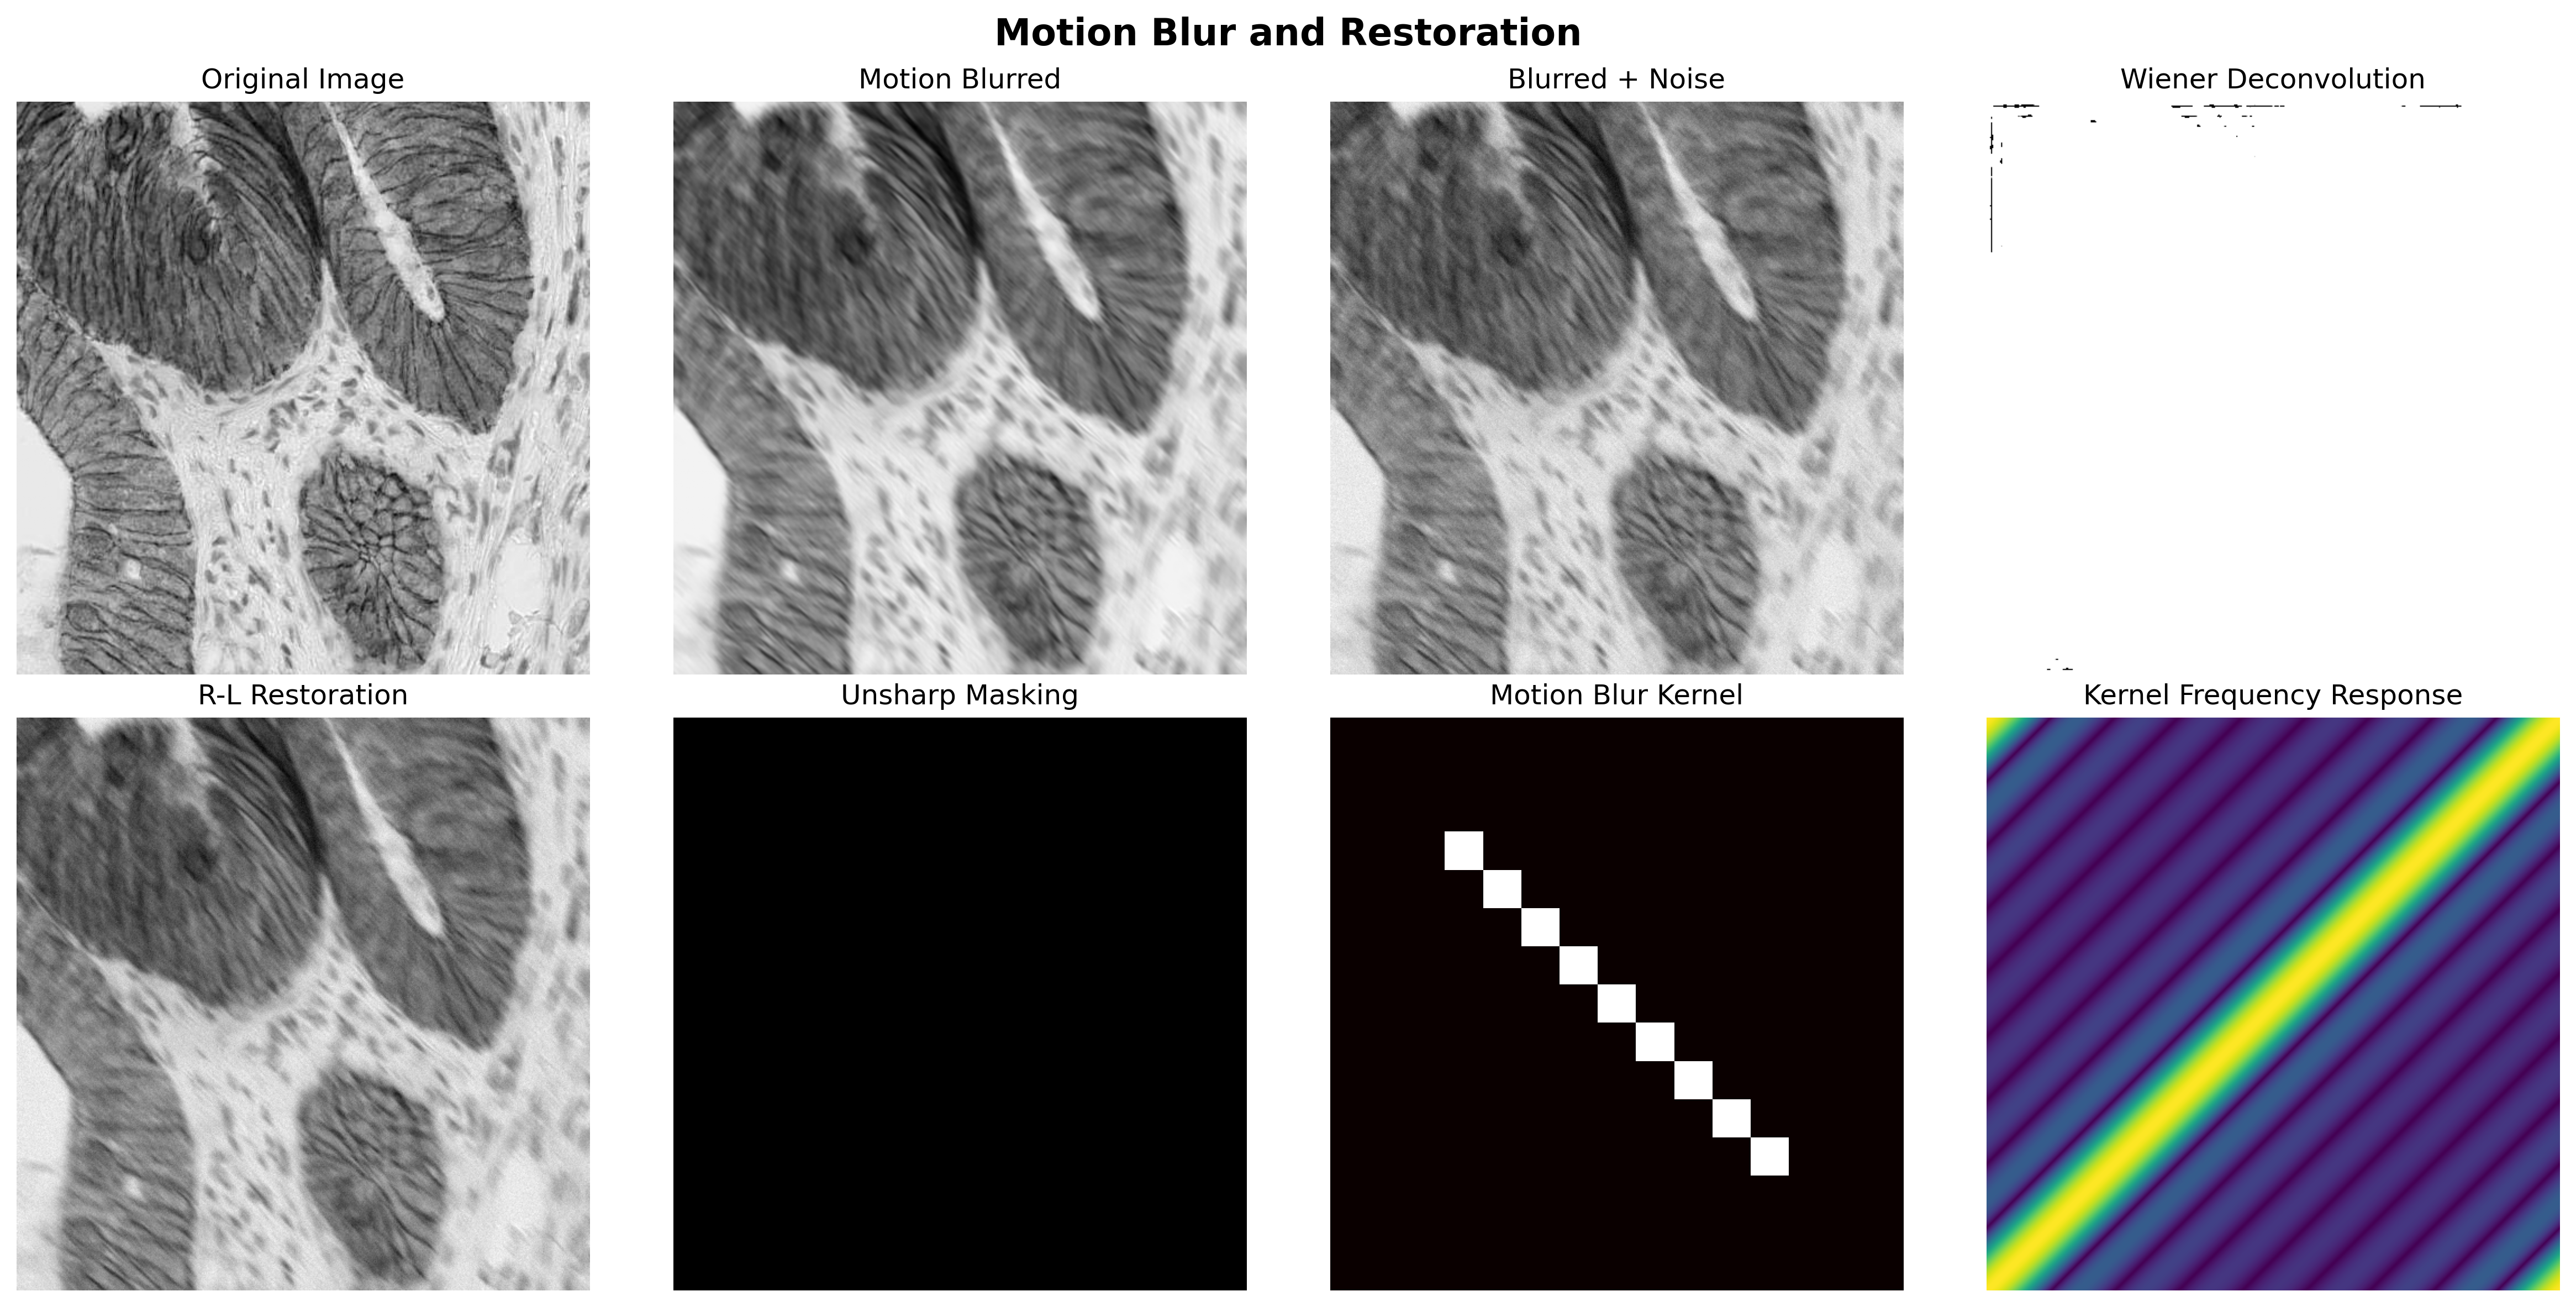
\includegraphics[width=\textwidth]{../figures/motion_blur_restoration.png}
        \end{column}
    \end{columns}
\end{frame}

\begin{frame}{Deblurring Techniques}
    \begin{columns}[T]
        \begin{column}{0.6\textwidth}
            \textbf{Richardson-Lucy Algorithm:}
            $$f^{(k+1)} = f^{(k)} \left[ h(-x,-y) * \frac{g}{h * f^{(k)}} \right]$$

            \textbf{Advantages:}
            \begin{itemize}
                \item Preserves positivity
                \item Iterative improvement
                \item Handles Poisson noise well
            \end{itemize}

            \textbf{Unsharp Masking:}
            $$f_{sharp} = f + \alpha(f - f_{blur})$$

            Where $f_{blur}$ is a low-pass filtered version of $f$.
        \end{column}
        \begin{column}{0.35\textwidth}
            \begin{insight}{Iteration Control}{}
                Stop Richardson-Lucy before noise amplification becomes dominant
            \end{insight}
        \end{column}
    \end{columns}
\end{frame}

\section{Image Inpainting}

\begin{frame}{Image Inpainting Overview}
    \begin{columns}[T]
        \begin{column}{0.6\textwidth}
            \textbf{Image Inpainting:} Fill in missing or damaged regions using information from surrounding areas.

            \textbf{Applications:}
            \begin{itemize}
                \item Object removal
                \item Restoration of damaged photographs
                \item Film restoration
                \item Text removal
            \end{itemize}

            \textbf{Key Challenges:}
            \begin{itemize}
                \item Preserving structural continuity
                \item Maintaining texture consistency
                \item Edge completion
            \end{itemize}
        \end{column}
        \begin{column}{0.35\textwidth}
            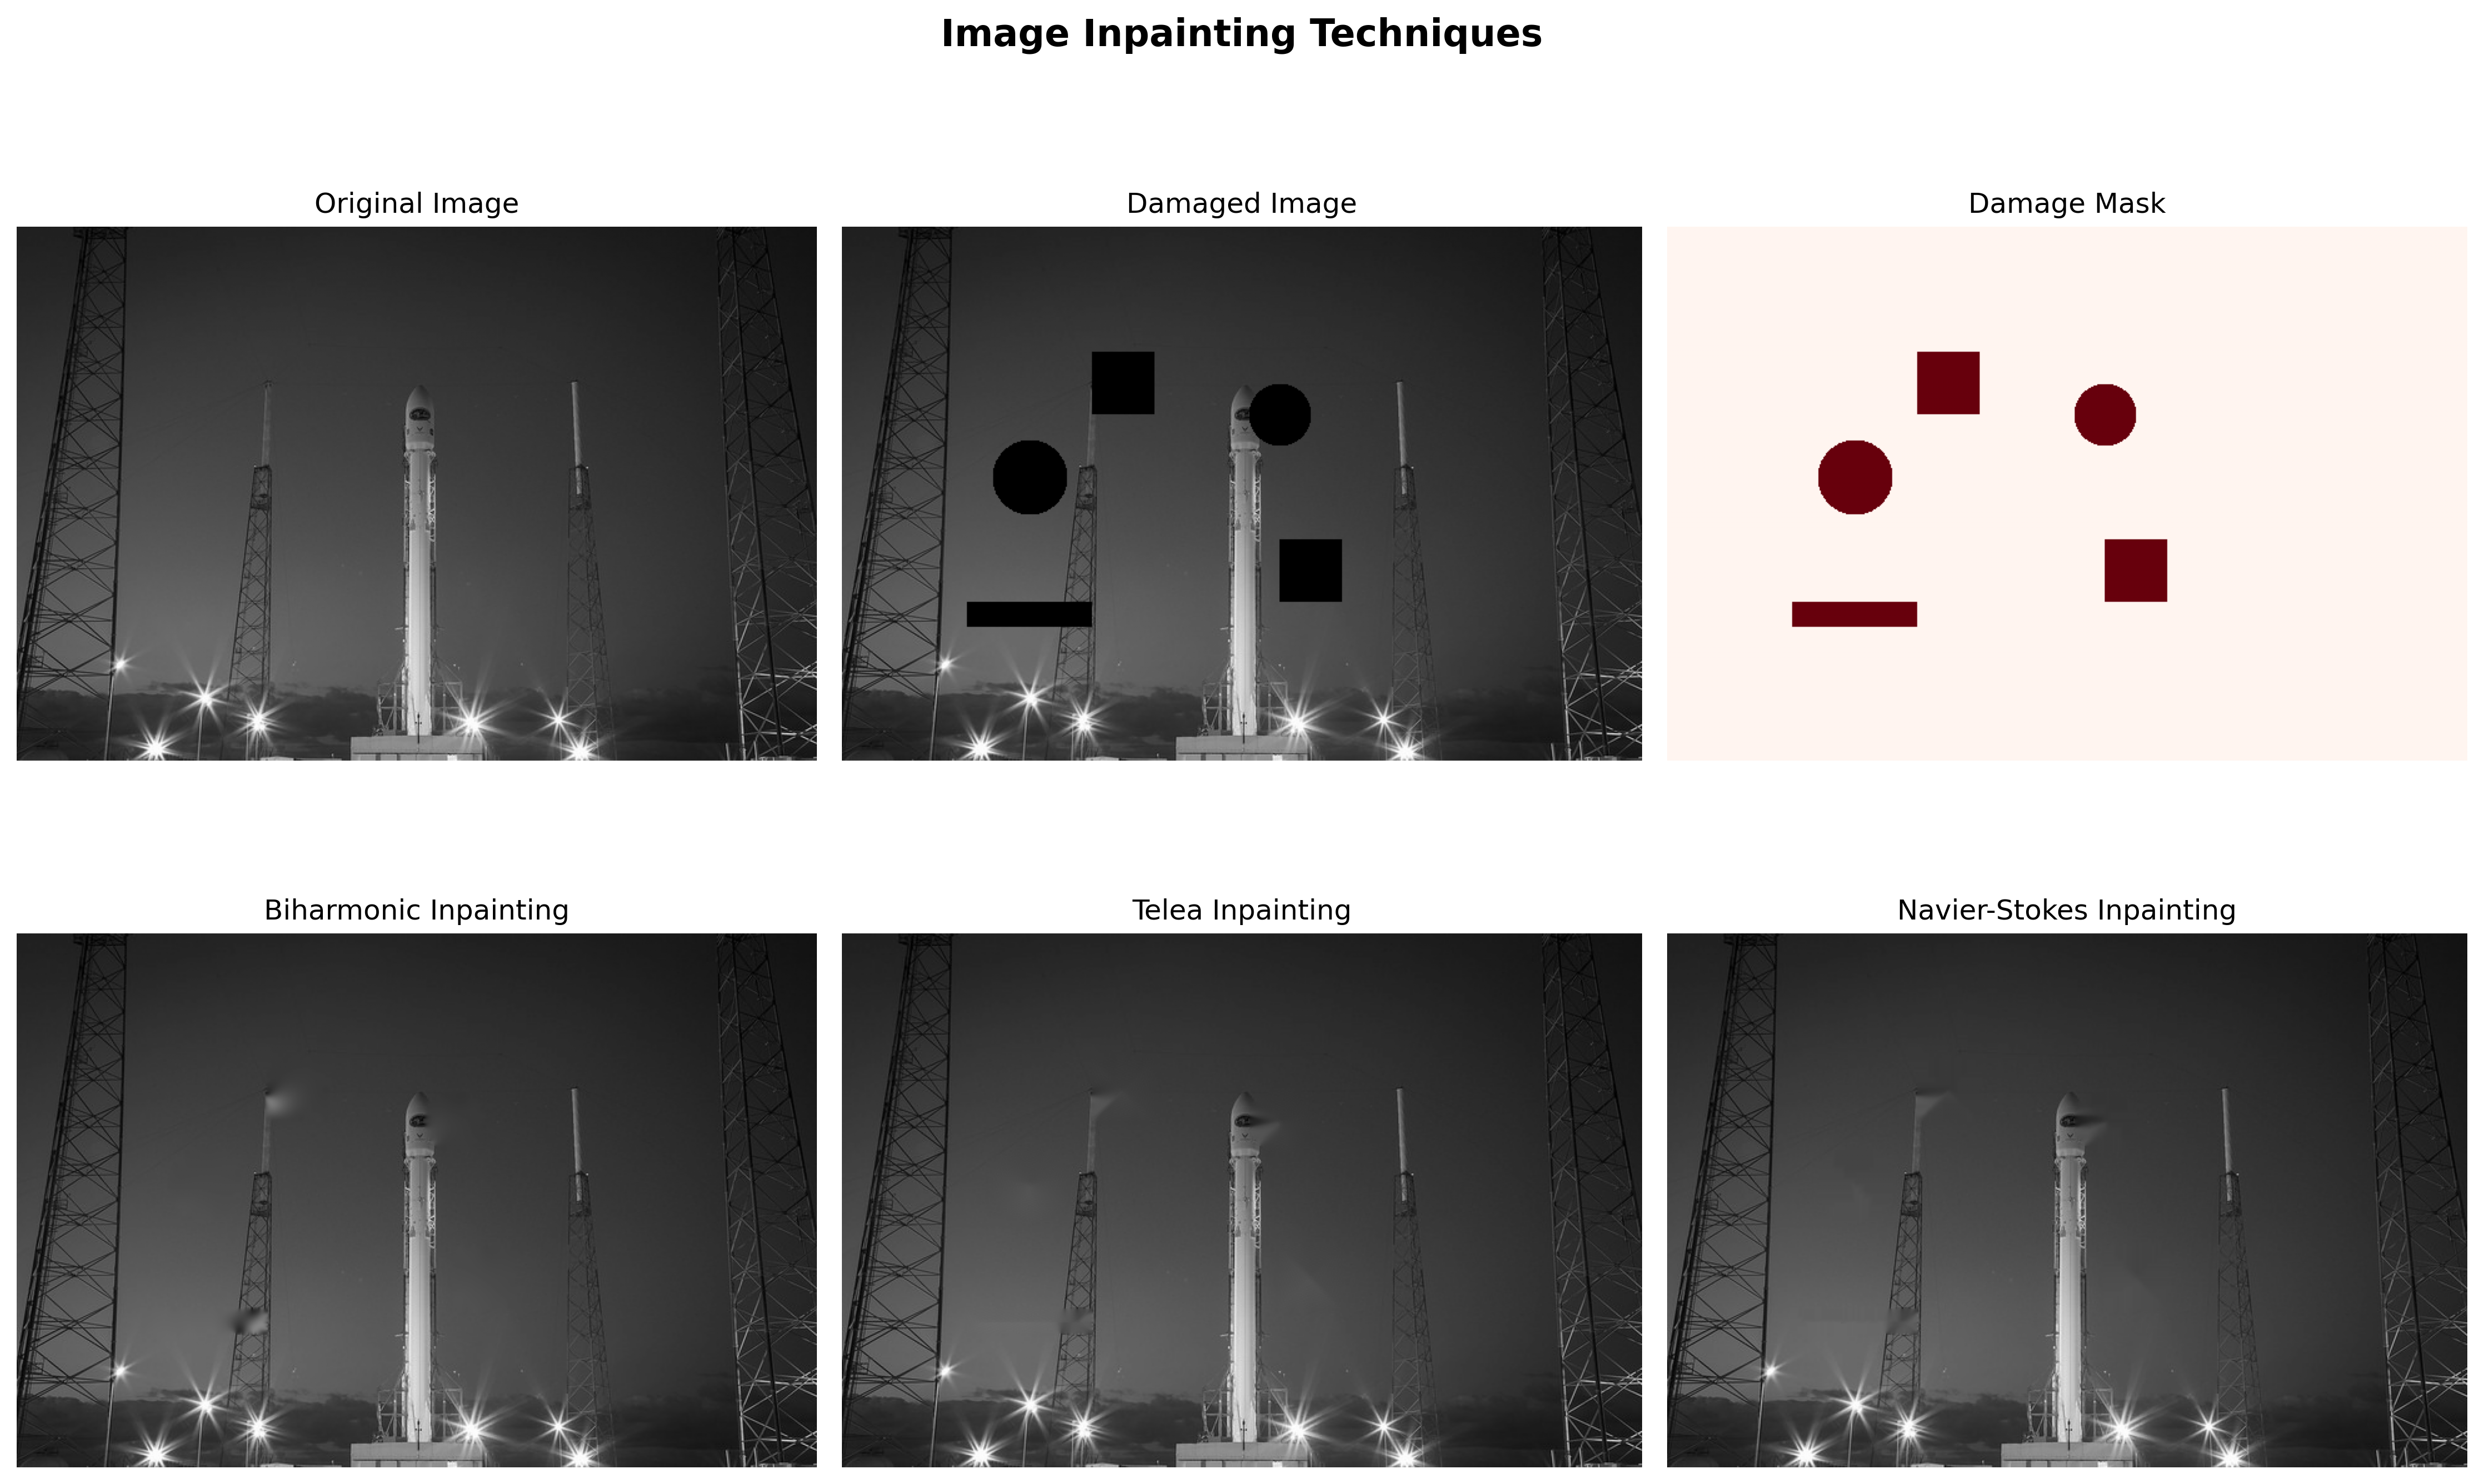
\includegraphics[width=\textwidth]{../figures/image_inpainting.png}
        \end{column}
    \end{columns}
\end{frame}

\begin{frame}{Inpainting Methods}
    \begin{columns}[T]
        \begin{column}{0.6\textwidth}
            \textbf{Biharmonic Inpainting:}
            Solves $\nabla^4 u = 0$ in the inpainting region with boundary conditions.

            \textbf{Telea Method:}
            Fast marching method using normalized weighted average:
            $$I(p) = \frac{\sum_{q \in B_\epsilon(p)} w(p,q) I(q)}{\sum_{q \in B_\epsilon(p)} w(p,q)}$$

            \textbf{Navier-Stokes Inpainting:}
            Uses fluid dynamics equations to propagate isophotes.

            \textbf{Selection Criteria:}
            \begin{itemize}
                \item Region size and shape
                \item Texture vs structure
                \item Computational requirements
            \end{itemize}
        \end{column}
        \begin{column}{0.35\textwidth}
            \begin{keypoint}{Inpainting Quality}{}
                Success depends on inpainting region size relative to surrounding texture period
            \end{keypoint}
        \end{column}
    \end{columns}
\end{frame}

\section{Geometric Processing}

\begin{frame}{Geometric Transformations}
    \begin{columns}[T]
        \begin{column}{0.6\textwidth}
            \textbf{Affine Transformations:}
            $$\begin{bmatrix} x' \\ y' \\ 1 \end{bmatrix} =
            \begin{bmatrix}
            a_{11} & a_{12} & a_{13} \\
            a_{21} & a_{22} & a_{23} \\
            0 & 0 & 1
            \end{bmatrix}
            \begin{bmatrix} x \\ y \\ 1 \end{bmatrix}$$

            \textbf{Basic Transformations:}
            \begin{itemize}
                \item Translation: $(x', y') = (x + t_x, y + t_y)$
                \item Rotation: $(x', y') = (x\cos\theta - y\sin\theta, x\sin\theta + y\cos\theta)$
                \item Scaling: $(x', y') = (s_x \cdot x, s_y \cdot y)$
                \item Shearing: $(x', y') = (x + sh_x \cdot y, y + sh_y \cdot x)$
            \end{itemize}
        \end{column}
        \begin{column}{0.35\textwidth}
            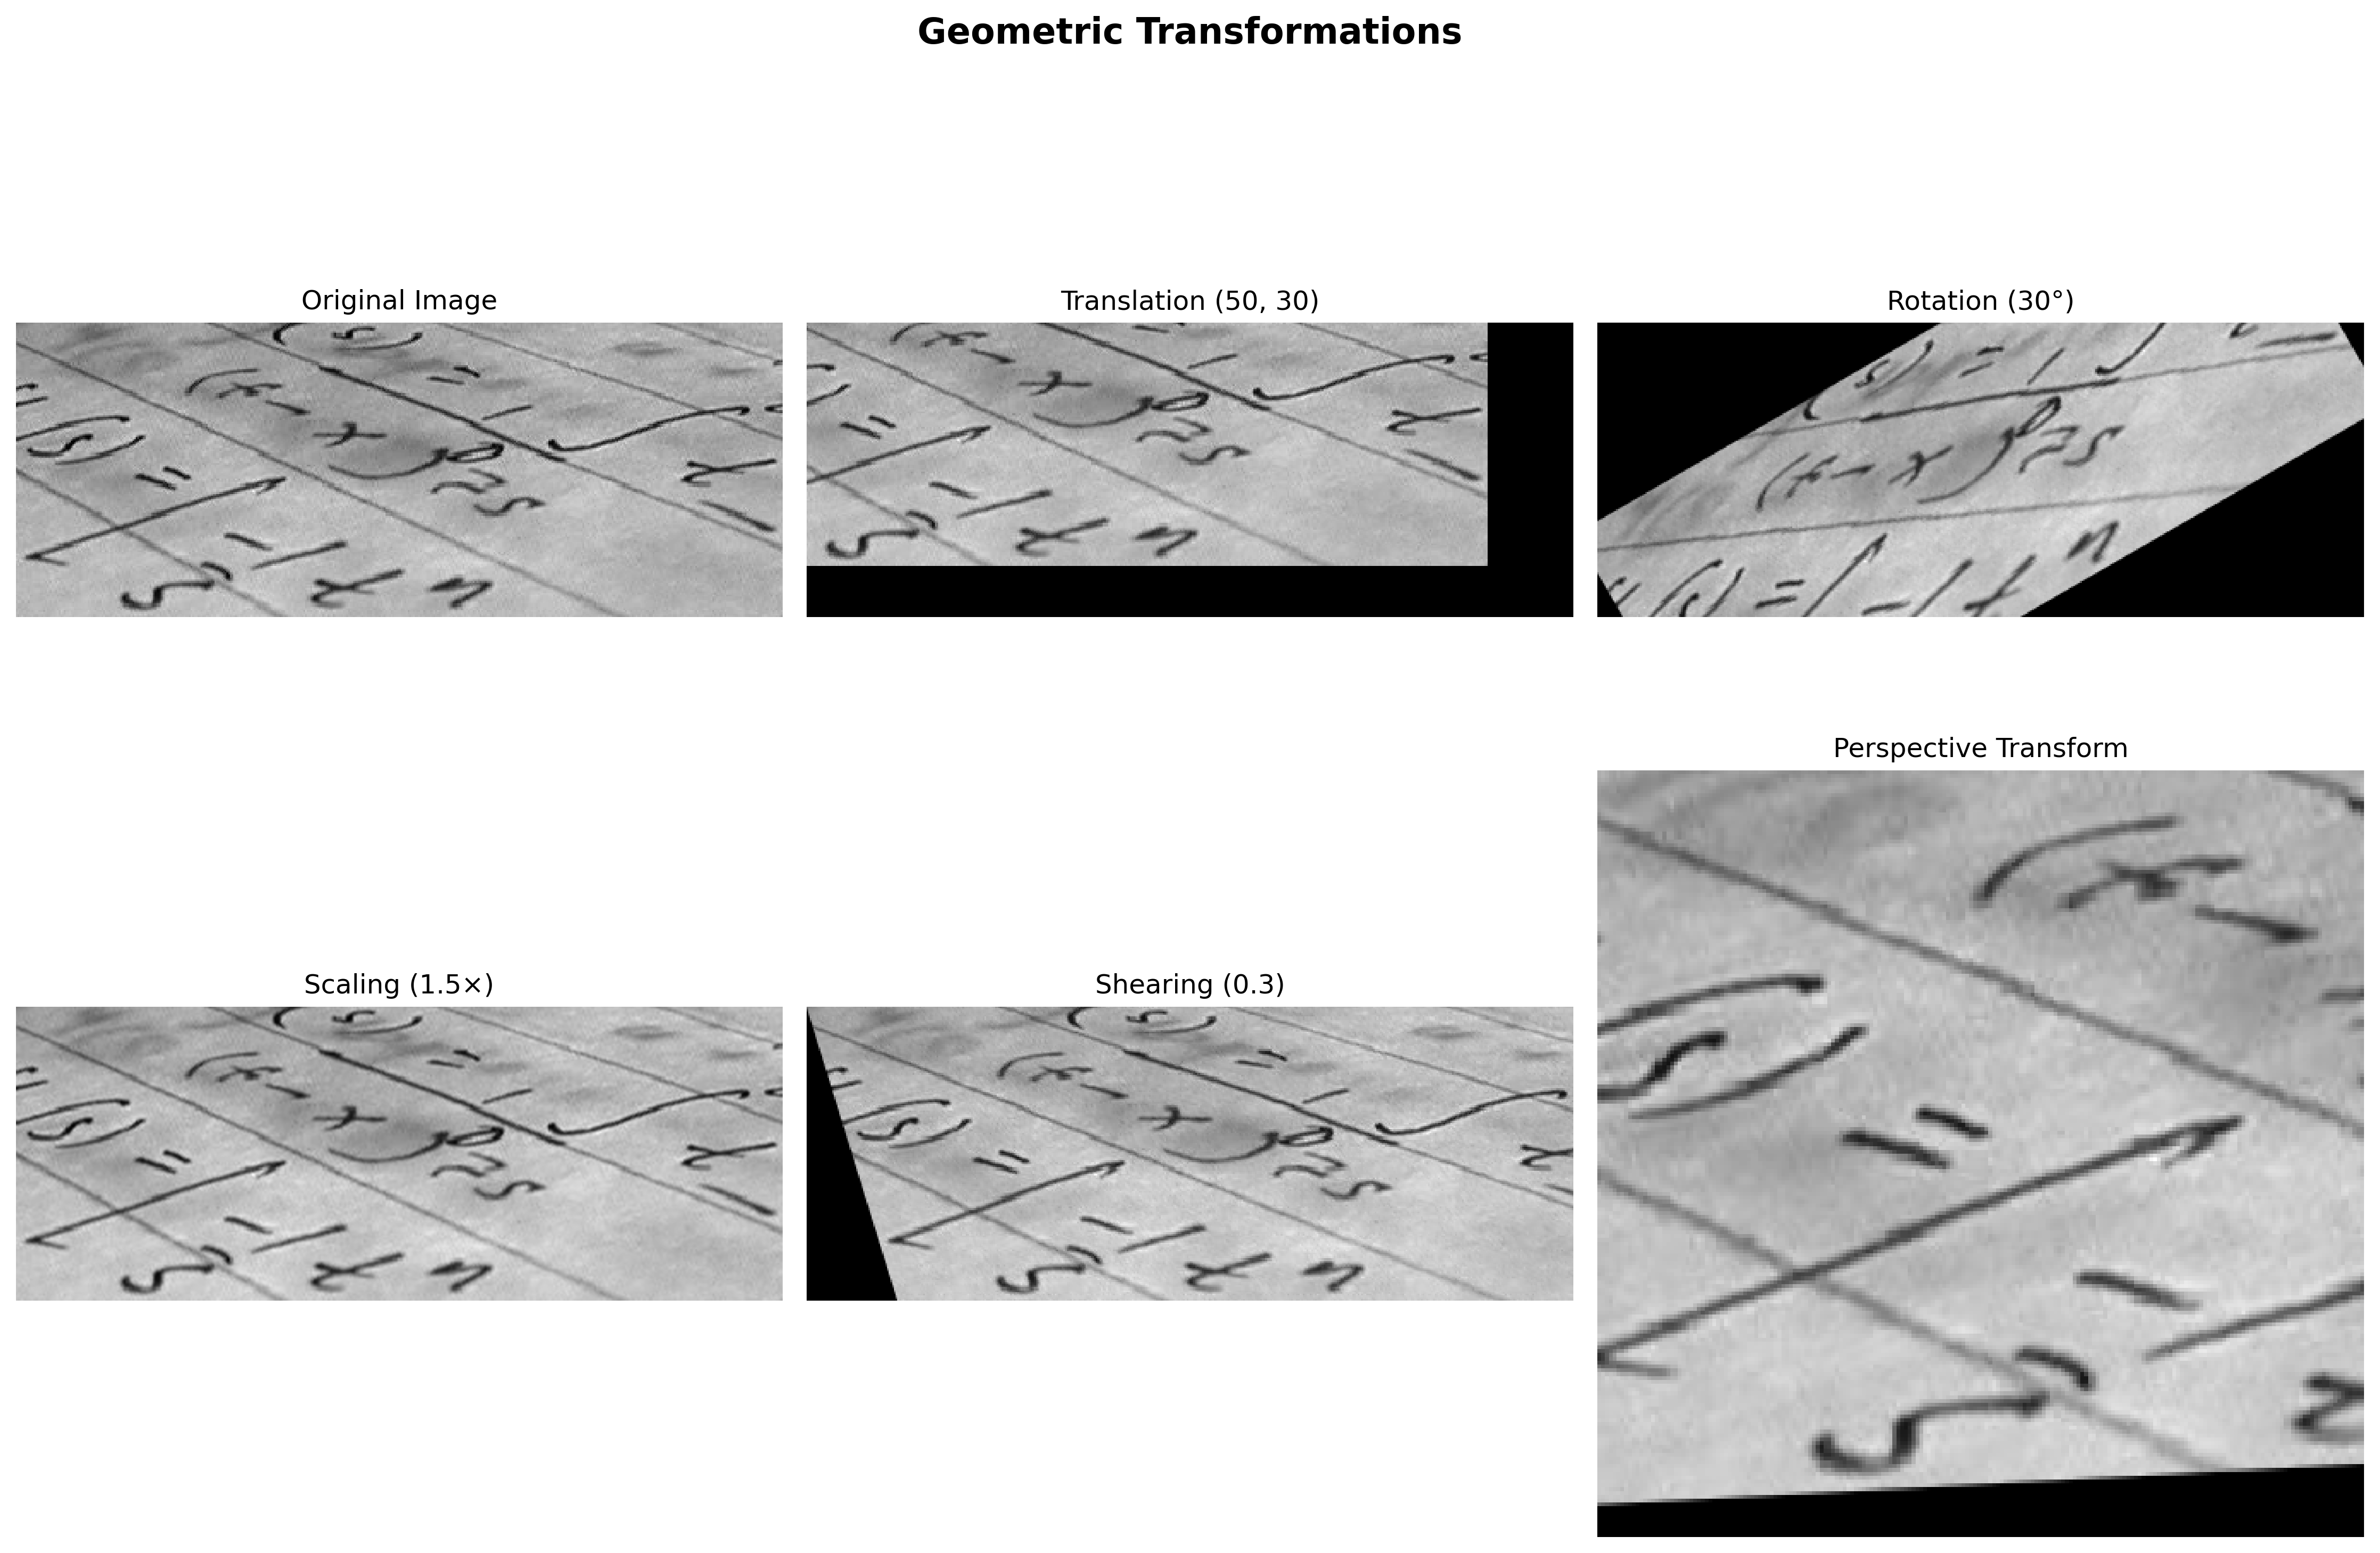
\includegraphics[width=\textwidth]{../figures/geometric_transformations.png}
        \end{column}
    \end{columns}
\end{frame}

\begin{frame}{Perspective and Projective Transformations}
    \begin{columns}[T]
        \begin{column}{0.6\textwidth}
            \textbf{Projective Transformation:}
            $$\begin{bmatrix} x' \\ y' \\ w' \end{bmatrix} =
            \begin{bmatrix}
            h_{11} & h_{12} & h_{13} \\
            h_{21} & h_{22} & h_{23} \\
            h_{31} & h_{32} & h_{33}
            \end{bmatrix}
            \begin{bmatrix} x \\ y \\ 1 \end{bmatrix}$$

            Where $(x', y') = (x'/w', y'/w')$

            \textbf{Properties:}
            \begin{itemize}
                \item Preserves collinearity
                \item Does not preserve parallelism
                \item 8 degrees of freedom
                \item Requires 4 point correspondences
            \end{itemize}
        \end{column}
        \begin{column}{0.35\textwidth}
            \begin{insight}{Homography}{}
                Perspective transformation is also called homography - useful for document rectification
            \end{insight}
        \end{column}
    \end{columns}
\end{frame}

\begin{frame}{Interpolation Methods}
    \begin{columns}[T]
        \begin{column}{0.6\textwidth}
            \textbf{Nearest Neighbor:}
            $$f(x,y) = f(\text{round}(x), \text{round}(y))$$

            \textbf{Bilinear Interpolation:}
            $$f(x,y) = \sum_{i=0}^{1}\sum_{j=0}^{1} f(x_i, y_j) \cdot l_i(x) \cdot l_j(y)$$

            \textbf{Bicubic Interpolation:}
            Uses 16 neighboring pixels with cubic polynomials.

            \textbf{Trade-offs:}
            \begin{itemize}
                \item Nearest: Fast, blocky artifacts
                \item Bilinear: Smooth, some blurring
                \item Bicubic: Best quality, most computation
            \end{itemize}
        \end{column}
        \begin{column}{0.35\textwidth}
            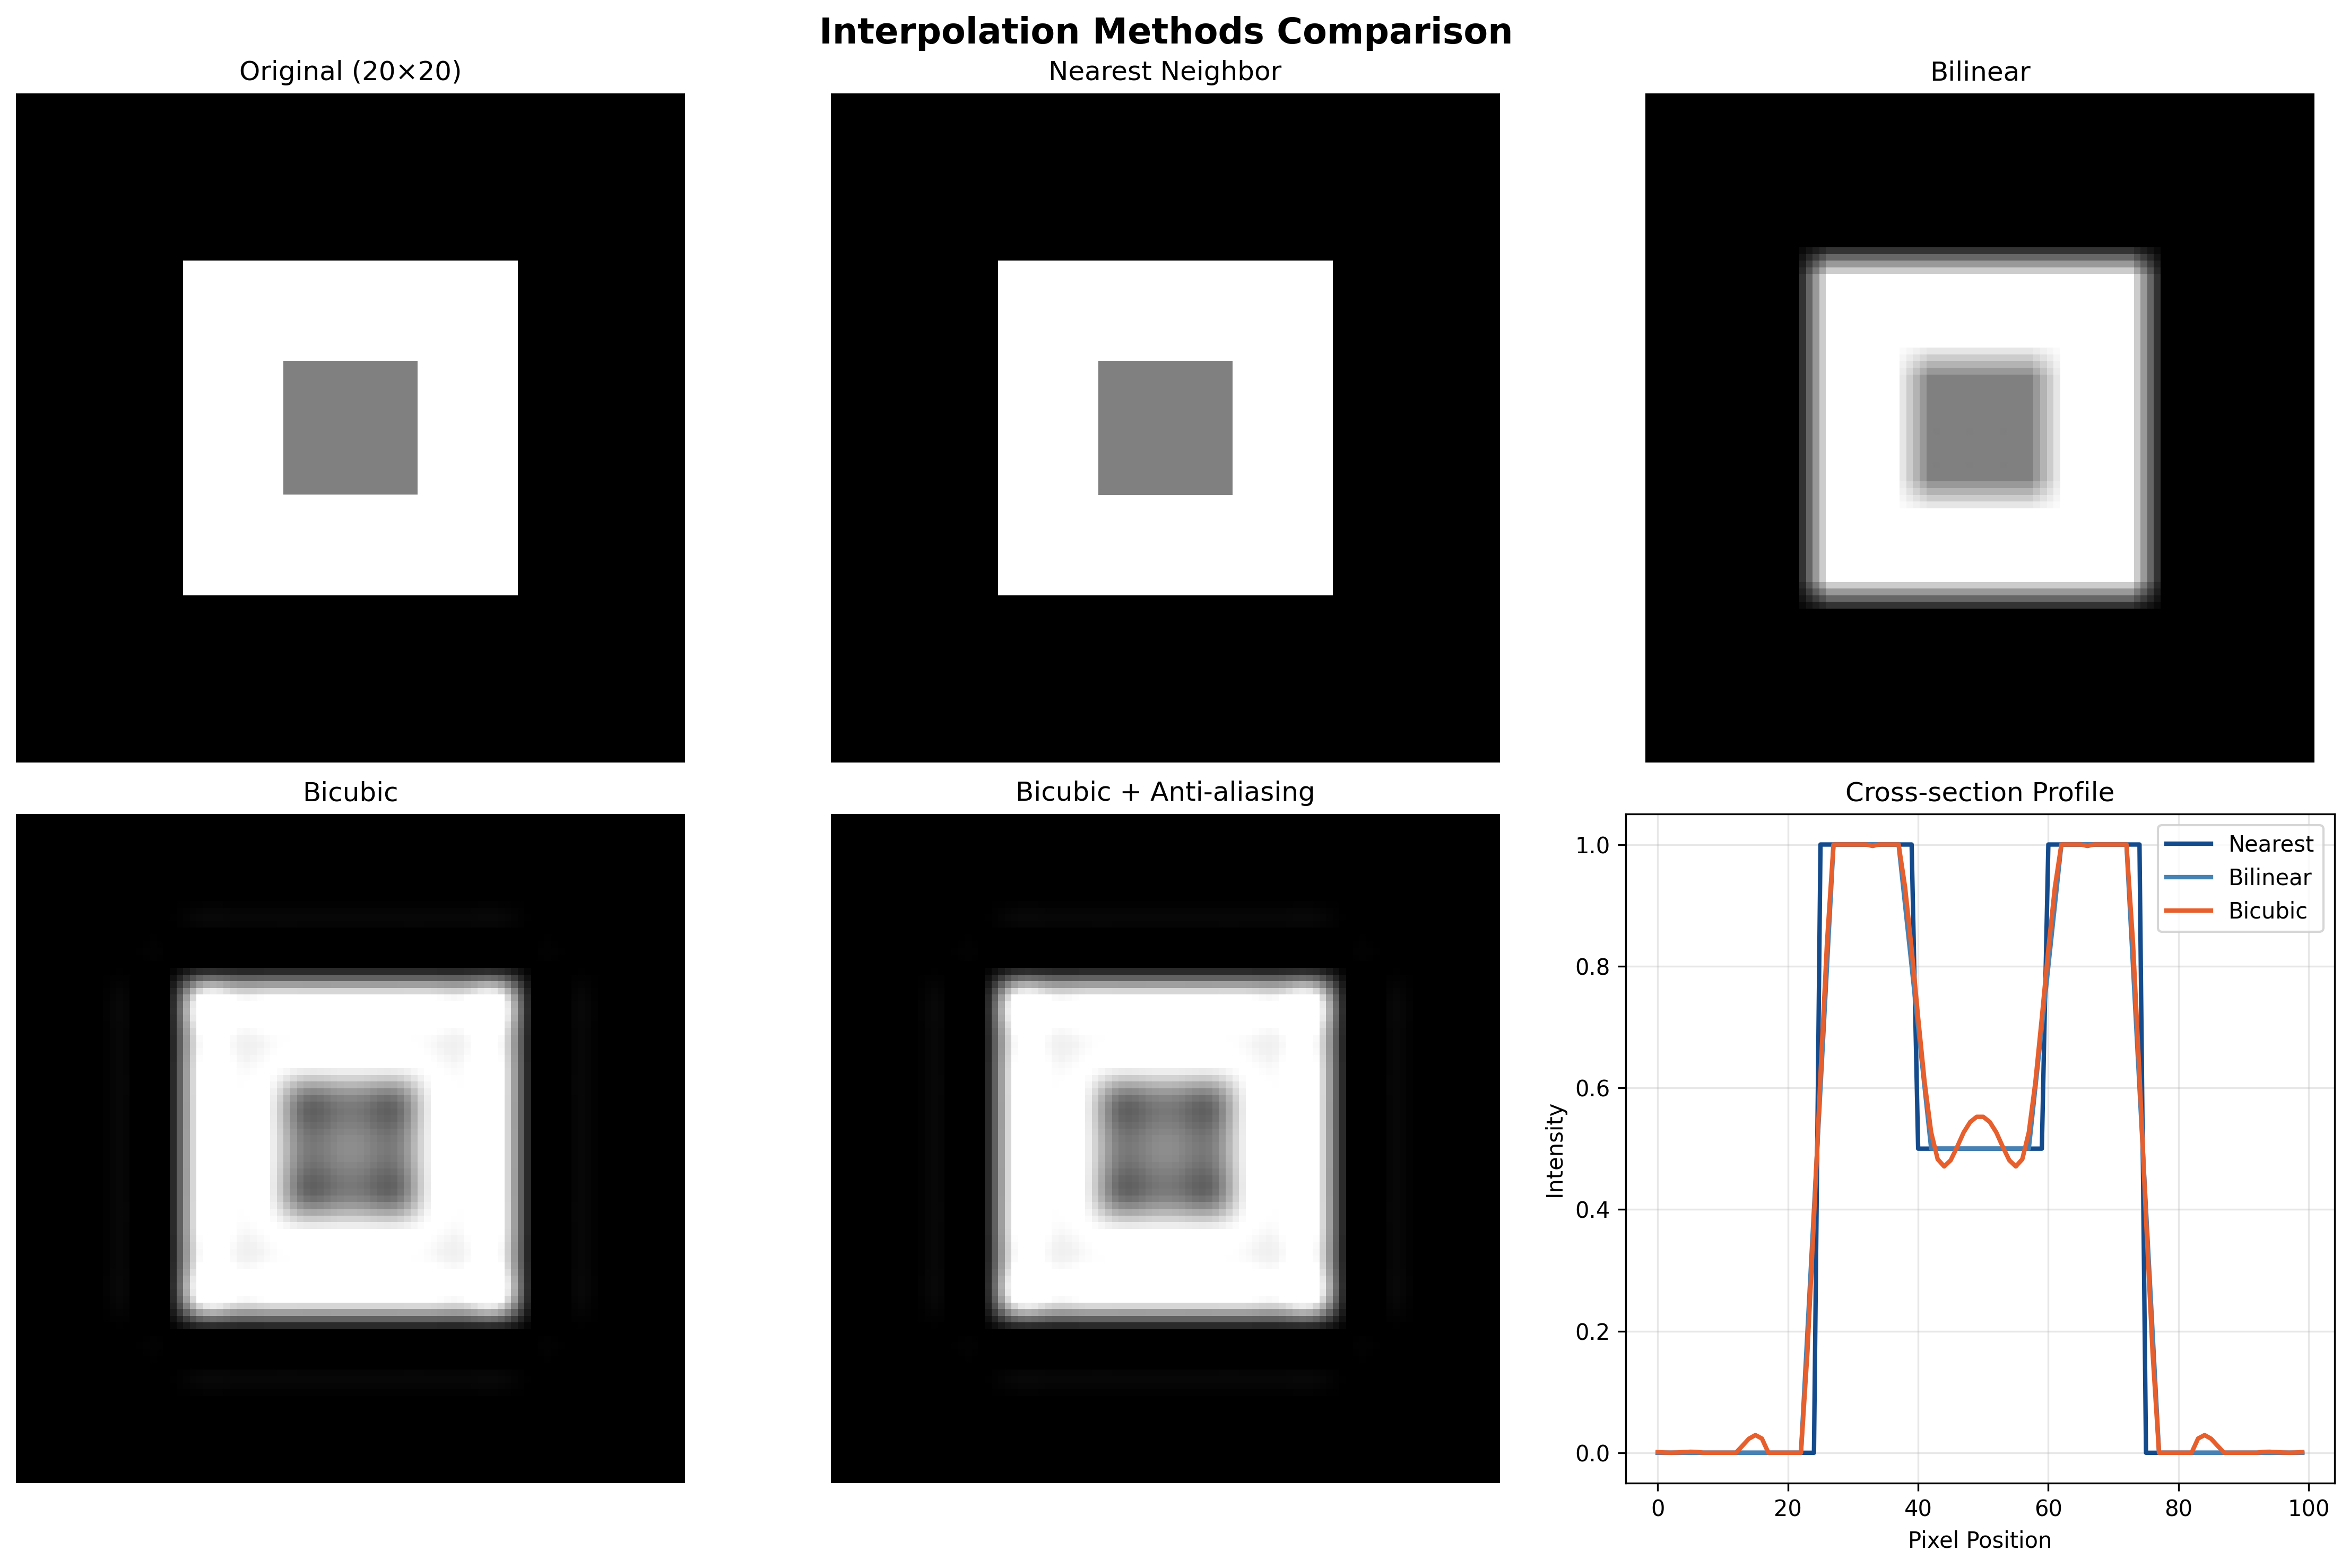
\includegraphics[width=\textwidth]{../figures/interpolation_methods.png}
        \end{column}
    \end{columns}
\end{frame}

\section{Advanced Techniques}

\begin{frame}{Non-local Means Denoising}
    \begin{columns}[T]
        \begin{column}{0.6\textwidth}
            \textbf{Non-local Means:}
            $$NL[u](x) = \frac{1}{C(x)} \int_\Omega w(x,y) u(y) dy$$

            Where the weight function is:
            $$w(x,y) = \exp\left(-\frac{||u(N_x) - u(N_y)||^2_{2,\sigma}}{h^2}\right)$$

            \textbf{Key Concepts:}
            \begin{itemize}
                \item $N_x$: Neighborhood around pixel $x$
                \item $h$: Filtering parameter
                \item $\sigma$: Standard deviation of Gaussian kernel
            \end{itemize}

            \textbf{Advantages:}
            \begin{itemize}
                \item Preserves textures and fine details
                \item Uses non-local information
                \item Effective for various noise types
            \end{itemize}
        \end{column}
        \begin{column}{0.35\textwidth}
            \begin{keypoint}{Non-local Philosophy}{}
                Similar patches can be found anywhere in the image, not just locally
            \end{keypoint}
        \end{column}
    \end{columns}
\end{frame}

\begin{frame}{Advanced Geometric Transformations}
    \begin{columns}[T]
        \begin{column}{0.6\textwidth}
            \textbf{Elastic Deformation:}
            Uses random displacement fields:
            $$\mathbf{d}(x,y) = \alpha \cdot G_\sigma * \mathbf{r}(x,y)$$

            Where $\mathbf{r}$ is random field and $G_\sigma$ is Gaussian filter.

            \textbf{Polar Transformations:}
            \begin{align}
            r &= \sqrt{x^2 + y^2} \\
            \theta &= \arctan(y/x)
            \end{align}

            \textbf{Applications:}
            \begin{itemize}
                \item Data augmentation
                \item Texture analysis
                \item Distortion correction
            \end{itemize}
        \end{column}
        \begin{column}{0.35\textwidth}
            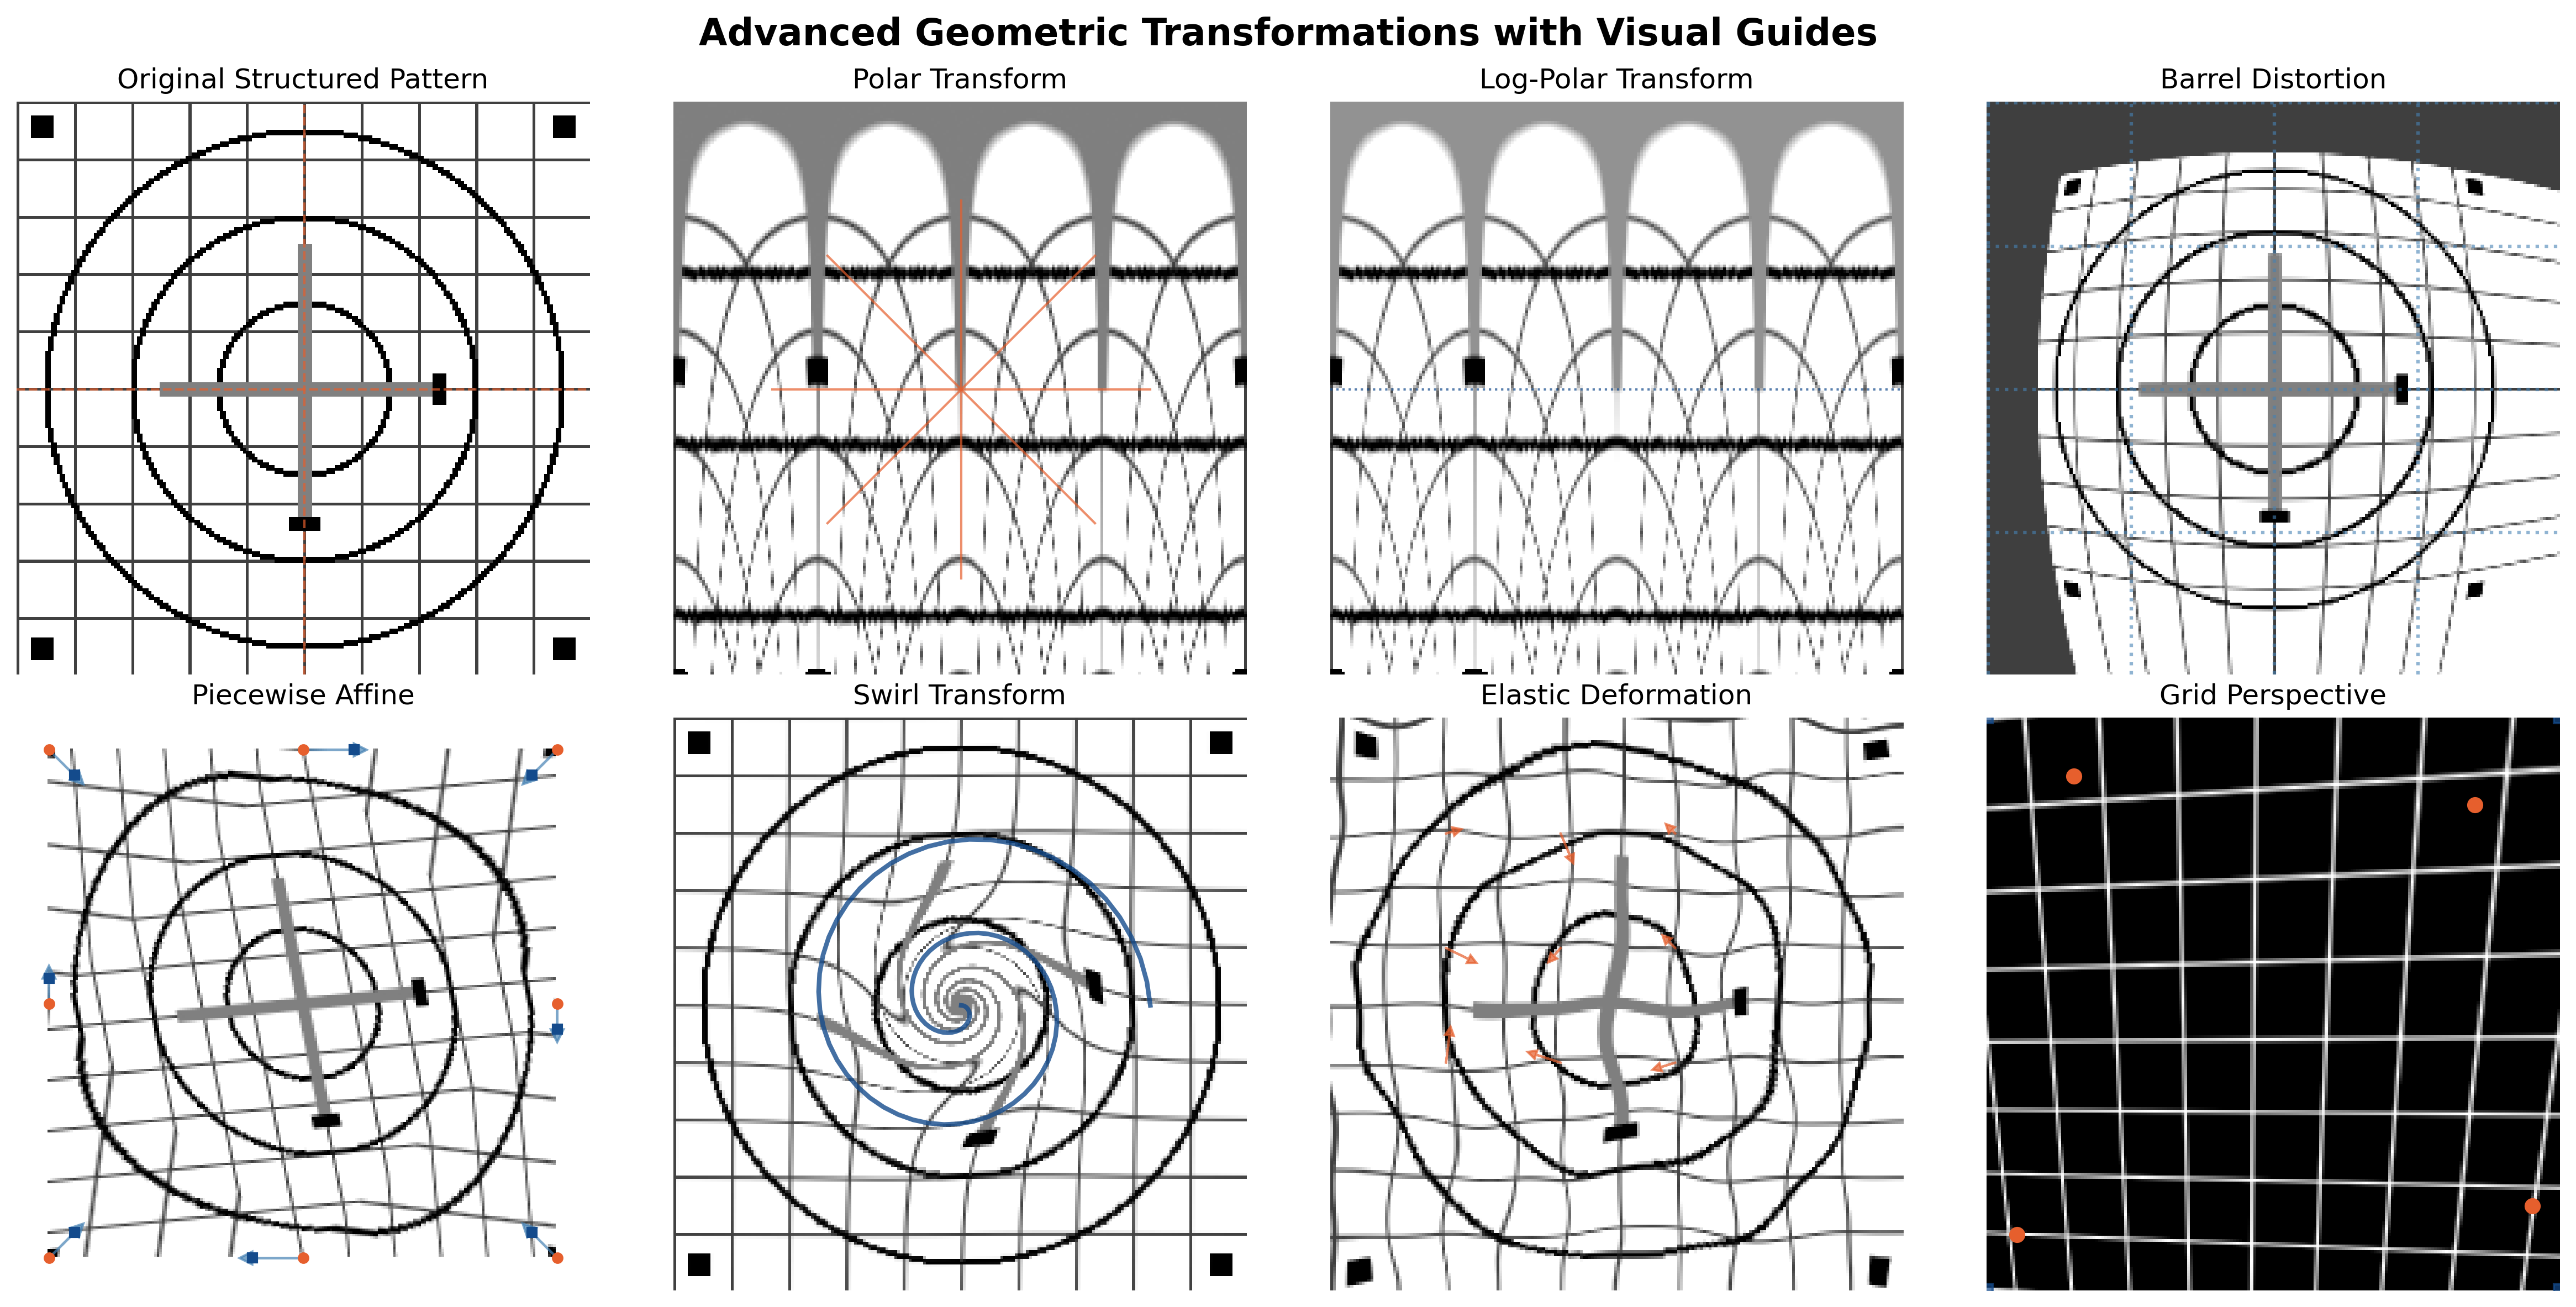
\includegraphics[width=\textwidth]{../figures/advanced_geometric_transforms.png}
        \end{column}
    \end{columns}
\end{frame}

\section{Real-World Applications}

\begin{frame}{Medical Image Restoration}
    \begin{columns}[T]
        \begin{column}{0.6\textwidth}
            \textbf{Common Issues in Medical Imaging:}
            \begin{itemize}
                \item Quantum noise (low dose)
                \item Ring artifacts (CT)
                \item Motion artifacts
                \item Beam hardening
            \end{itemize}

            \textbf{Specialized Techniques:}
            \begin{itemize}
                \item Anisotropic diffusion
                \item Total variation denoising
                \item Iterative reconstruction
                \item Wavelet denoising
            \end{itemize}

            \textbf{Quality Requirements:}
            \begin{itemize}
                \item Preserve diagnostic features
                \item Quantitative accuracy
                \item No false artifacts
            \end{itemize}
        \end{column}
        \begin{column}{0.35\textwidth}
            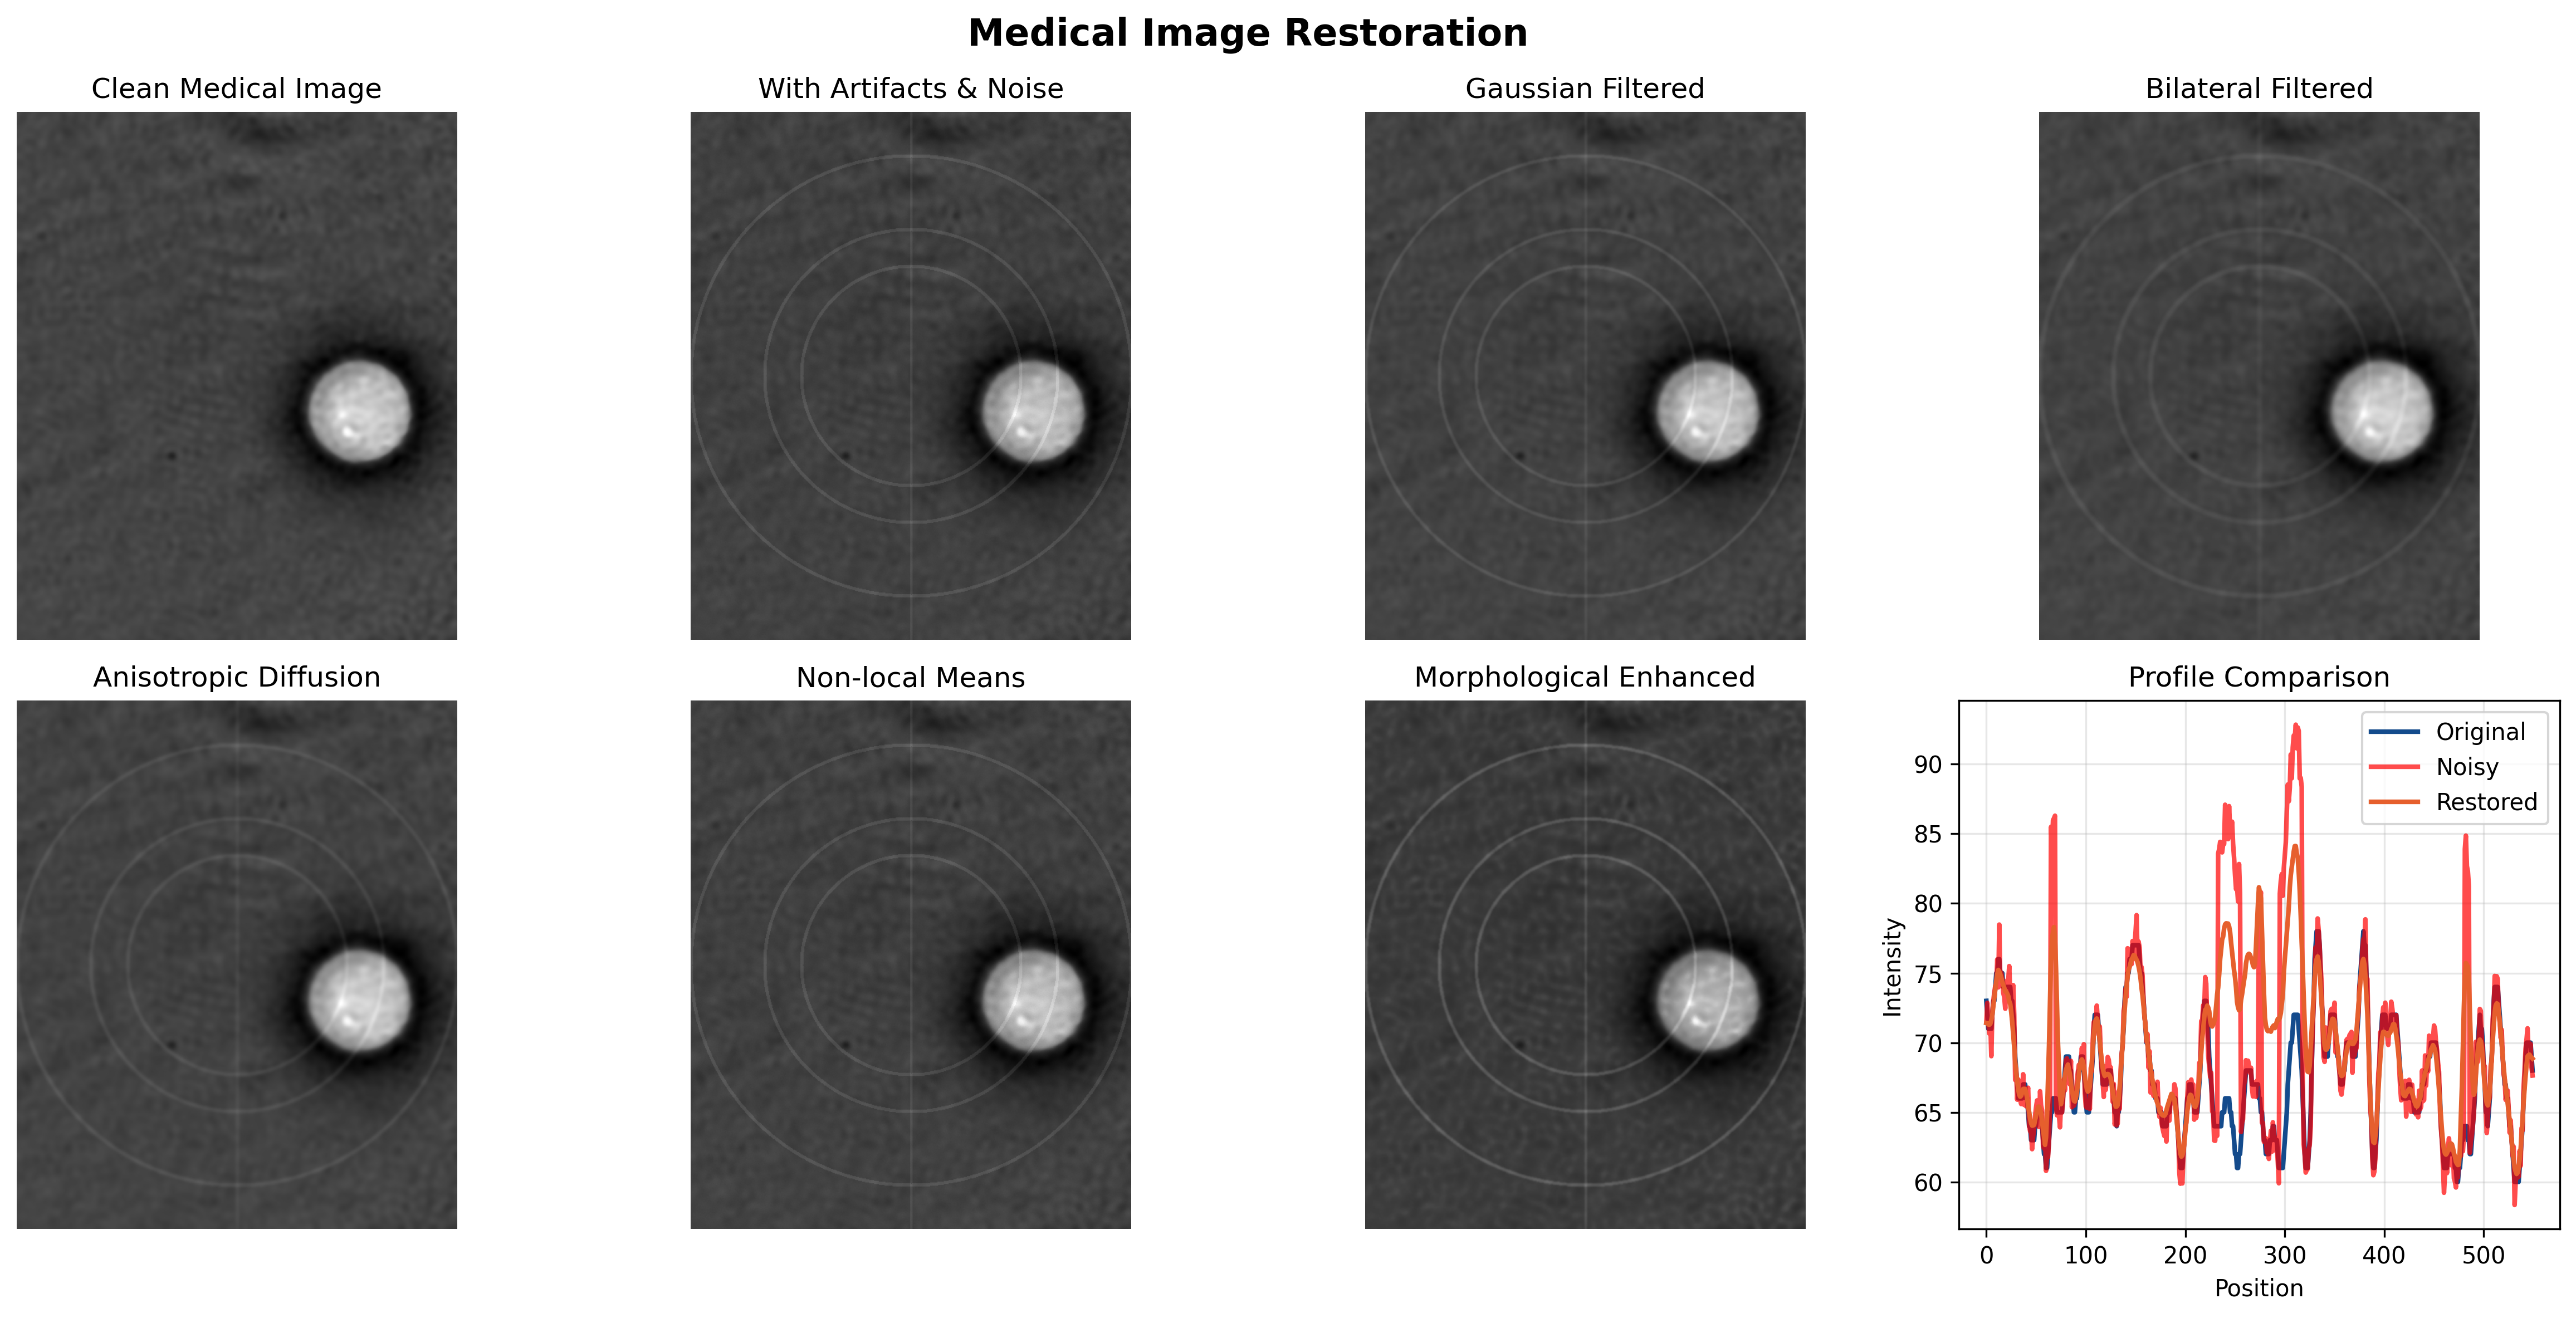
\includegraphics[width=\textwidth]{../figures/medical_image_restoration.png}
        \end{column}
    \end{columns}
\end{frame}

\begin{frame}{Document Processing}
    \begin{columns}[T]
        \begin{column}{0.6\textwidth}
            \textbf{Document Processing Pipeline:}
            \begin{enumerate}
                \item Deskewing and orientation correction
                \item Noise reduction
                \item Binarization
                \item Character enhancement
            \end{enumerate}

            \textbf{Geometric Corrections:}
            \begin{itemize}
                \item Perspective correction
                \item Barrel/pincushion distortion
                \item Page curvature correction
            \end{itemize}

            \textbf{OCR Preprocessing:}
            \begin{itemize}
                \item Connected component analysis
                \item Morphological operations
                \item Skew detection and correction
            \end{itemize}
        \end{column}
        \begin{column}{0.35\textwidth}
            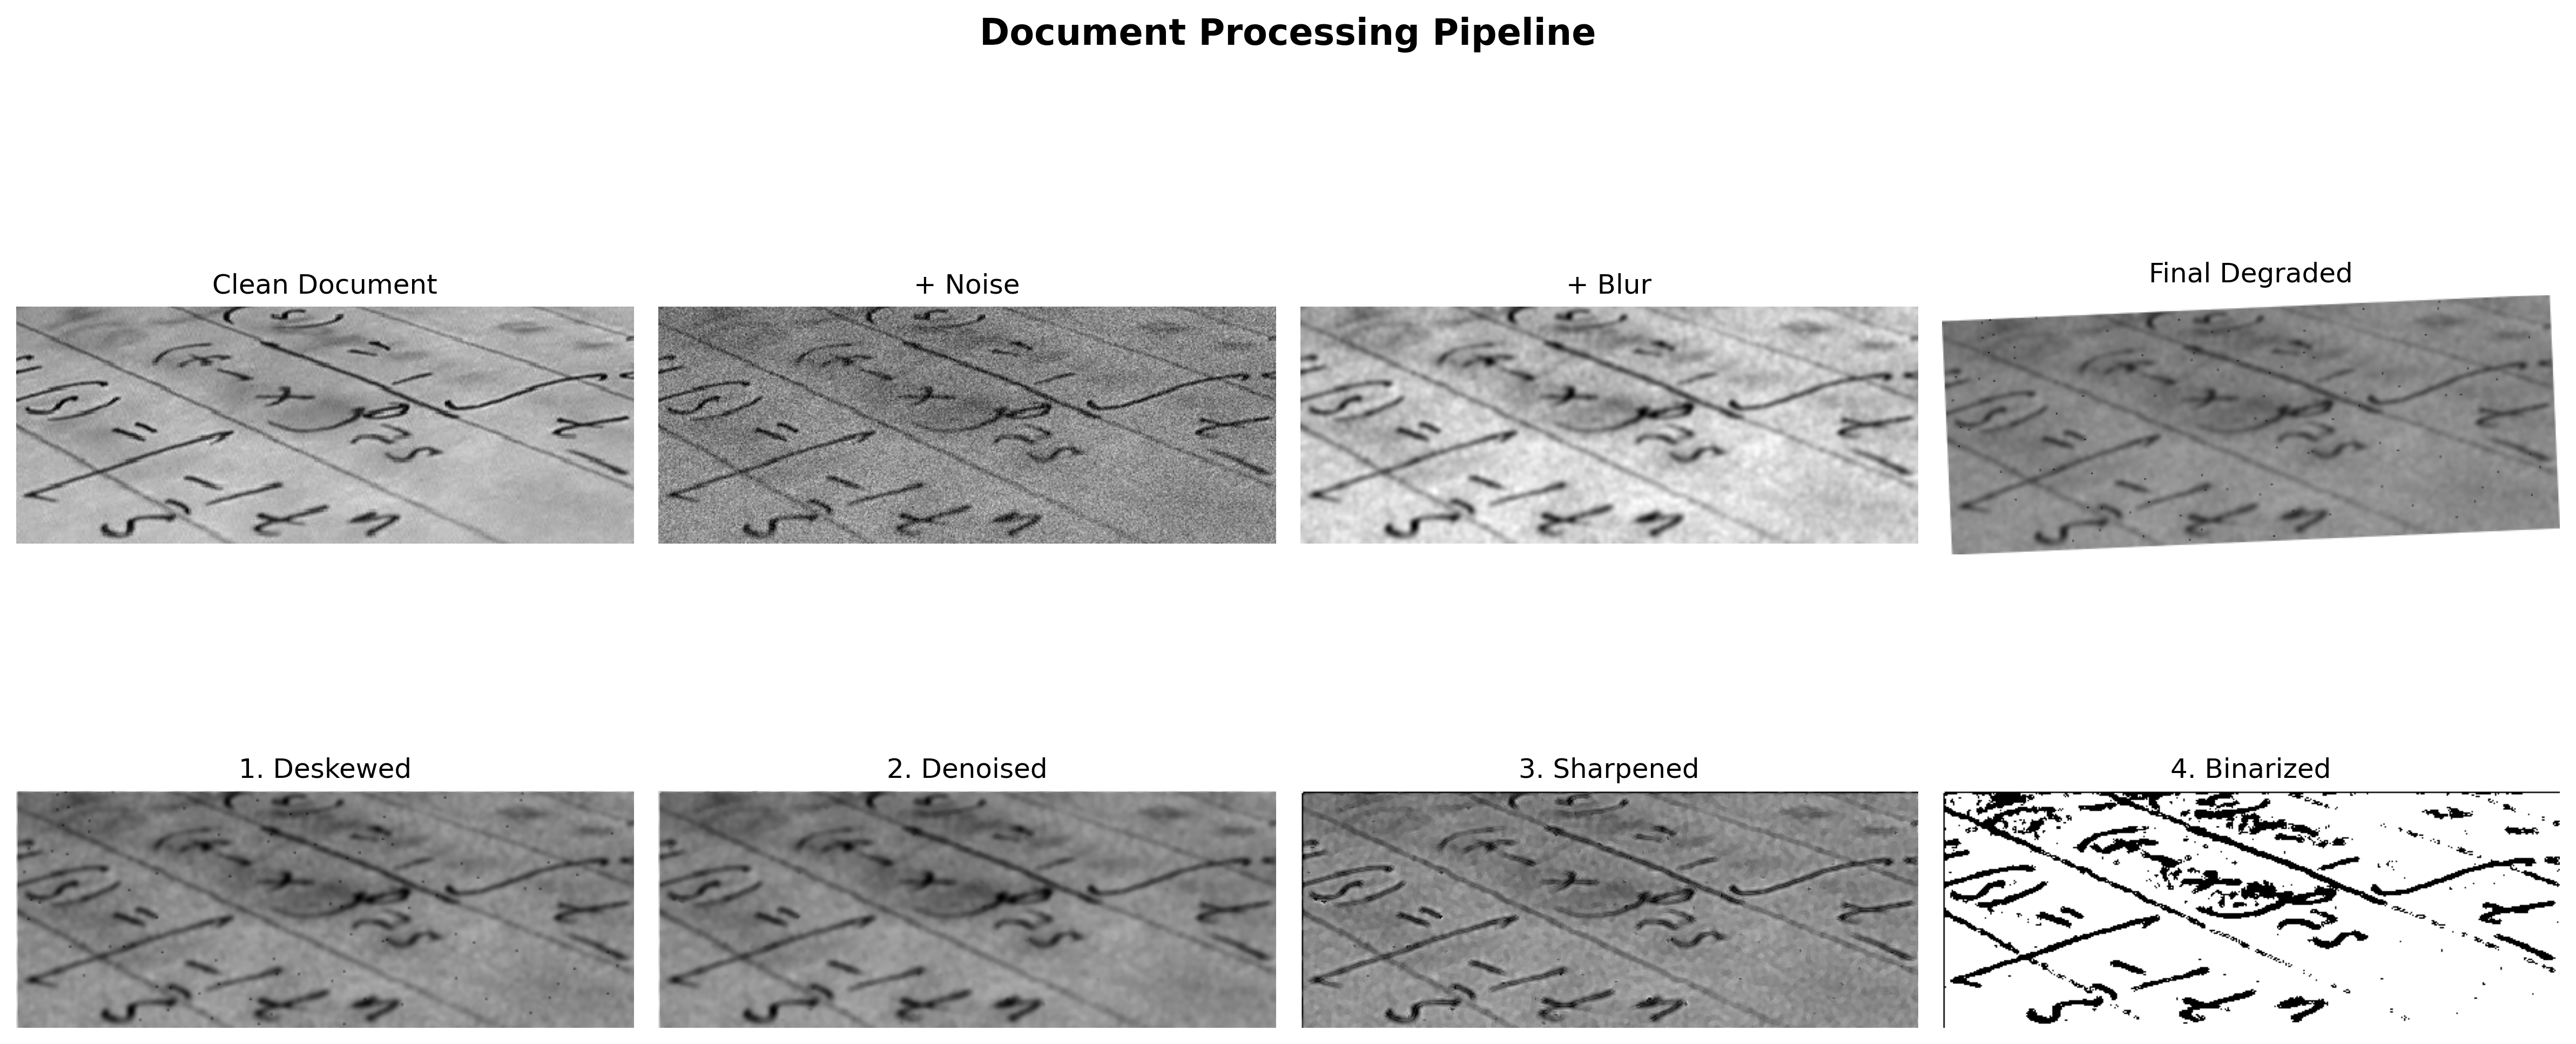
\includegraphics[width=\textwidth]{../figures/document_processing.png}
        \end{column}
    \end{columns}
\end{frame}

\begin{frame}{Computer Vision Preprocessing}
    \begin{columns}[T]
        \begin{column}{0.6\textwidth}
            \textbf{Preprocessing for Object Detection:}
            \begin{enumerate}
                \item Illumination normalization
                \item Noise reduction
                \item Contrast enhancement
                \item Geometric normalization
            \end{enumerate}

            \textbf{Registration Applications:}
            \begin{itemize}
                \item Multi-temporal analysis
                \item Stereo vision
                \item Medical image fusion
                \item Panorama stitching
            \end{itemize}

            \textbf{Quality Metrics:}
            \begin{itemize}
                \item Feature detectability
                \item Registration accuracy
                \item Computational efficiency
            \end{itemize}
        \end{column}
        \begin{column}{0.35\textwidth}
            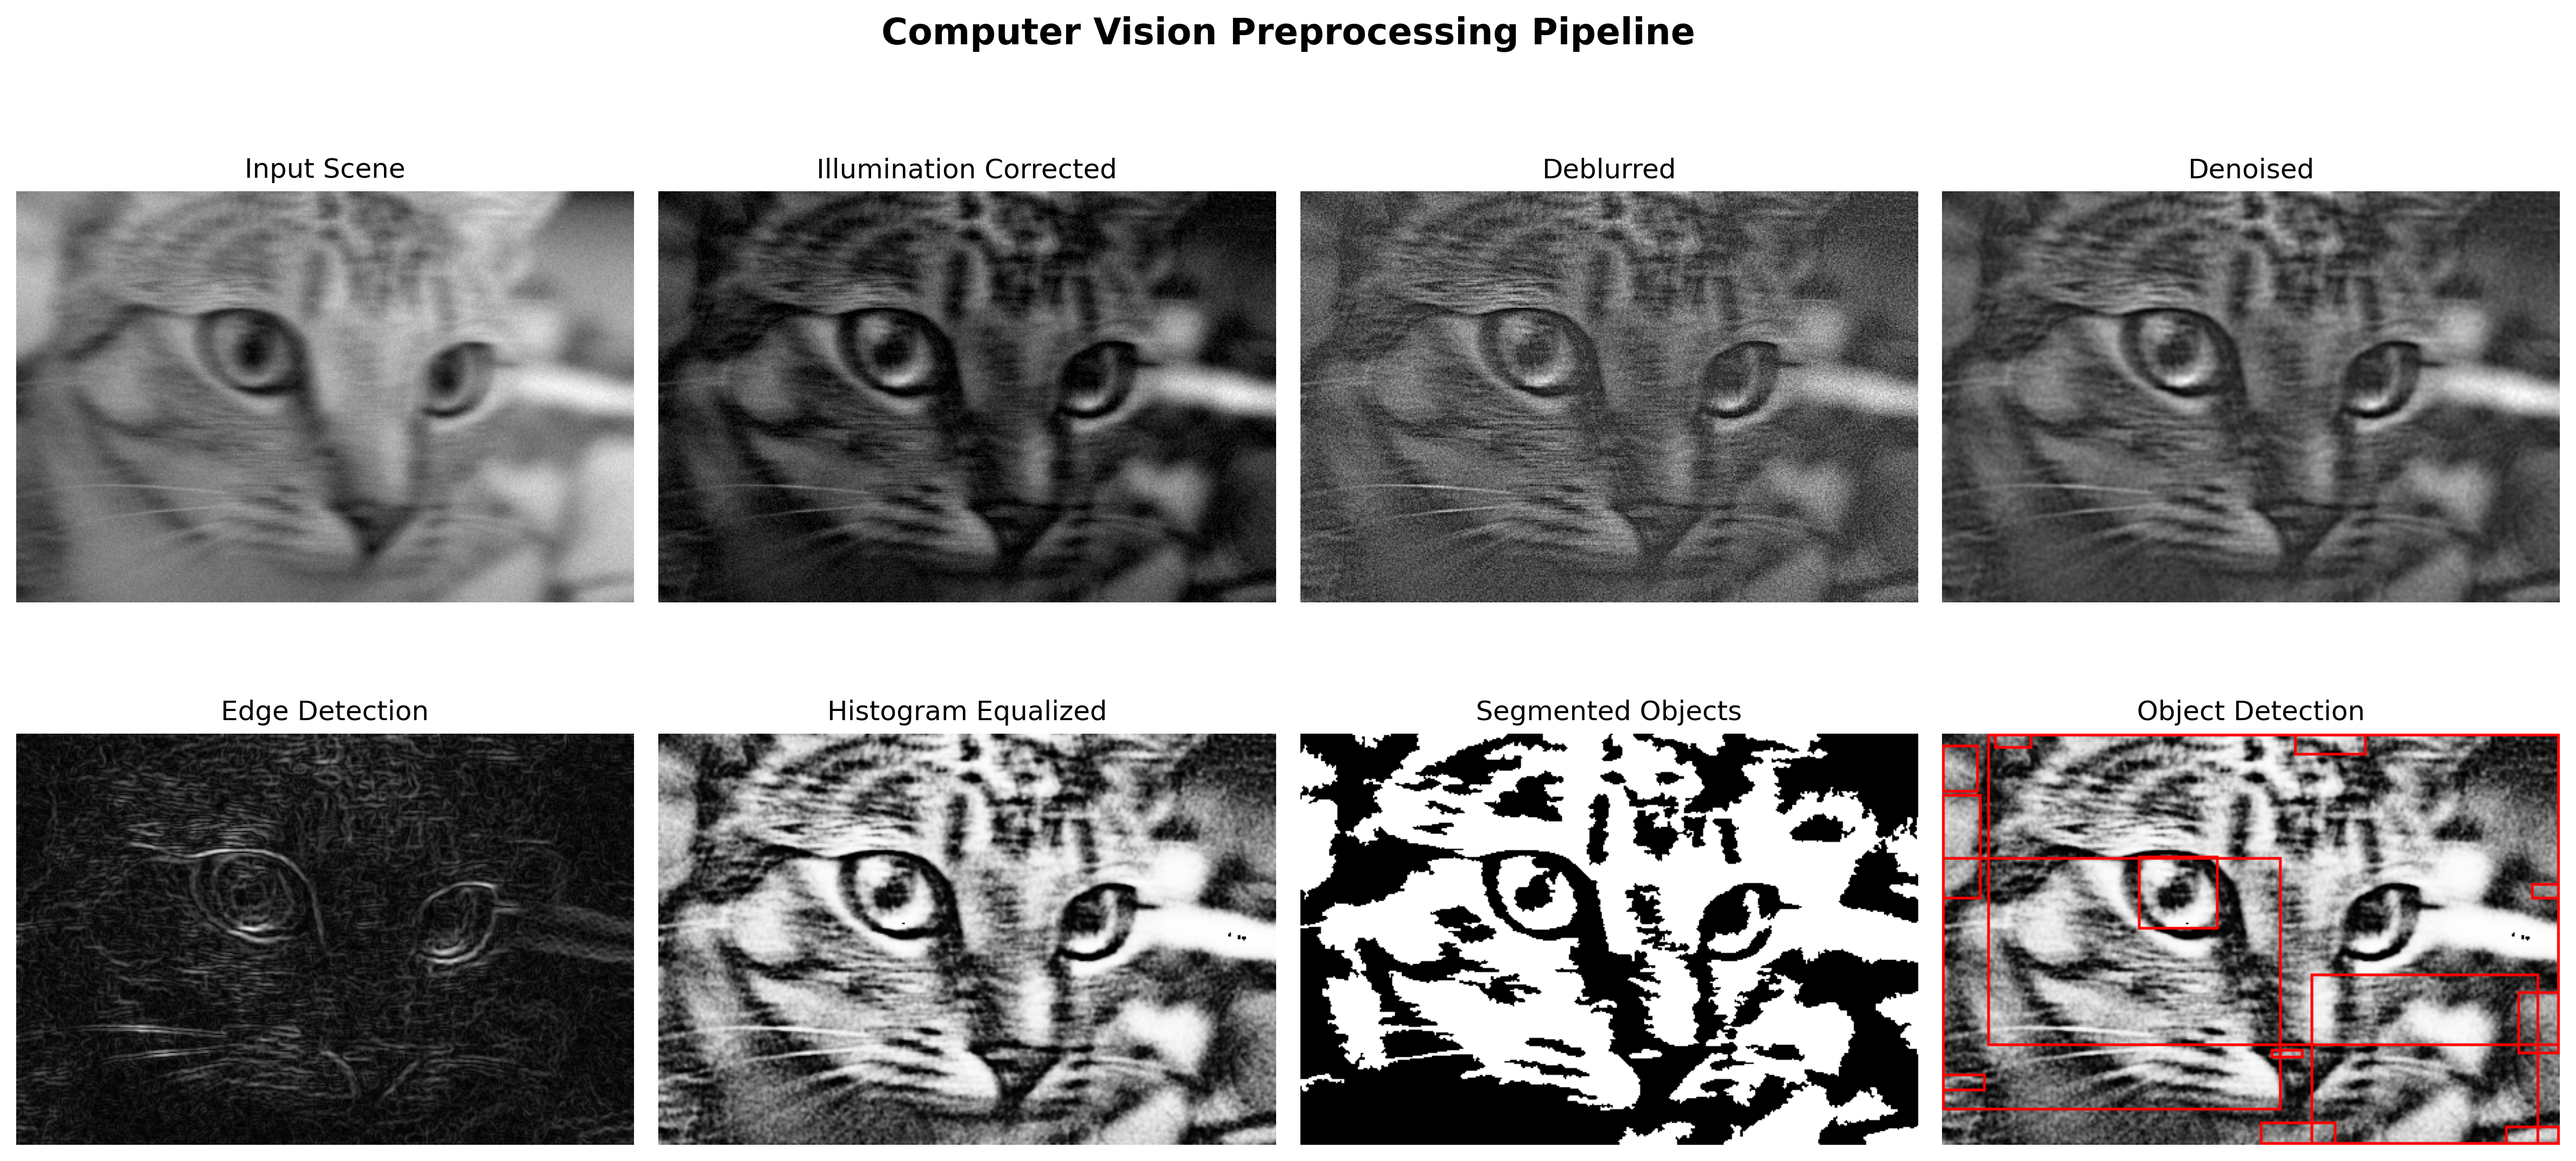
\includegraphics[width=\textwidth]{../figures/computer_vision_preprocessing.png}
        \end{column}
    \end{columns}
\end{frame}

\section{Quality Assessment}

\begin{frame}{Restoration Quality Metrics}
    \begin{columns}[T]
        \begin{column}{0.6\textwidth}
            \textbf{Peak Signal-to-Noise Ratio (PSNR):}
            $$\text{PSNR} = 10 \log_{10} \frac{MAX_I^2}{\text{MSE}}$$

            Where $\text{MSE} = \frac{1}{mn}\sum_{i=0}^{m-1}\sum_{j=0}^{n-1}[I(i,j) - K(i,j)]^2$

            \textbf{Structural Similarity Index (SSIM):}
            $$\text{SSIM}(x,y) = \frac{(2\mu_x\mu_y + c_1)(2\sigma_{xy} + c_2)}{(\mu_x^2 + \mu_y^2 + c_1)(\sigma_x^2 + \sigma_y^2 + c_2)}$$

            \textbf{Mean Structural Similarity (MSSIM):}
            $$\text{MSSIM}(X,Y) = \frac{1}{M}\sum_{j=1}^{M} \text{SSIM}(x_j, y_j)$$
        \end{column}
        \begin{column}{0.35\textwidth}
            
\includegraphics[width=\textwidth]{../figures/quality_metrics.png}
        \end{column}
    \end{columns}
\end{frame}

\begin{frame}{No-Reference Quality Assessment}
    \begin{columns}[T]
        \begin{column}{0.6\textwidth}
            \textbf{When Original is Unknown:}
            \begin{itemize}
                \item Blind/no-reference metrics
                \item Statistical measures
                \item Perceptual quality metrics
            \end{itemize}

            \textbf{Common NR Metrics:}
            \begin{itemize}
                \item Total Variation (TV)
                \item Gradient magnitude
                \item Laplacian energy
                \item Entropy measures
            \end{itemize}

            \textbf{Perceptual Metrics:}
            \begin{itemize}
                \item BRISQUE (Blind/Referenceless Image Spatial Quality Evaluator)
                \item NIQE (Natural Image Quality Evaluator)
                \item Deep learning-based metrics
            \end{itemize}
        \end{column}
        \begin{column}{0.35\textwidth}
            \begin{insight}{Quality Trade-offs}{}
                Higher PSNR doesn't always mean better perceptual quality
            \end{insight}
        \end{column}
    \end{columns}
\end{frame}

\section{Best Practices and Pitfalls}

\begin{frame}{Common Pitfalls in Restoration}
    \begin{columns}[T]
        \begin{column}{0.6\textwidth}
            \textbf{Algorithmic Pitfalls:}
            \begin{itemize}
                \item Over-restoration (removing important details)
                \item Under-restoration (insufficient improvement)
                \item Ringing artifacts from inverse filtering
                \item Boundary effects in frequency domain
            \end{itemize}

            \textbf{Parameter Selection Issues:}
            \begin{itemize}
                \item Inappropriate filter parameters
                \item Wrong noise model assumptions
                \item Insufficient iteration control
                \item Poor regularization balance
            \end{itemize}

            \textbf{Computational Considerations:}
            \begin{itemize}
                \item Numerical precision issues
                \item Memory requirements for large images
                \item Convergence criteria
            \end{itemize}
        \end{column}
        \begin{column}{0.35\textwidth}
            \begin{keypoint}{Validation Importance}{}
                Always validate restoration results with ground truth or expert assessment
            \end{keypoint}
        \end{column}
    \end{columns}
\end{frame}

\begin{frame}{Best Practices}
    \begin{columns}[T]
        \begin{column}{0.6\textwidth}
            \textbf{Pre-processing Guidelines:}
            \begin{itemize}
                \item Characterize degradation model
                \item Estimate noise parameters
                \item Choose appropriate restoration method
                \item Consider computational constraints
            \end{itemize}

            \textbf{Parameter Tuning:}
            \begin{itemize}
                \item Use cross-validation when possible
                \item Start with conservative parameters
                \item Monitor quality metrics during processing
                \item Compare multiple methods
            \end{itemize}

            \textbf{Post-processing:}
            \begin{itemize}
                \item Validate results quantitatively
                \item Check for artifacts
                \item Consider perceptual quality
                \item Document parameter choices
            \end{itemize}
        \end{column}
        \begin{column}{0.35\textwidth}
            \begin{insight}{Method Selection}{}
                No single method works best for all types of degradation
            \end{insight}
        \end{column}
    \end{columns}
\end{frame}

\section{Summary and Future Directions}

\begin{frame}{Key Takeaways}
    \textbf{Image Restoration Fundamentals:}
    \begin{itemize}
        \item Degradation model understanding is crucial
        \item Multiple approaches: spatial, frequency, iterative
        \item Quality assessment guides method selection
    \end{itemize}

    \textbf{Geometric Processing:}
    \begin{itemize}
        \item Transform hierarchy: rigid → affine → projective
        \item Interpolation method affects final quality
        \item Registration enables many applications
    \end{itemize}

    \textbf{Practical Considerations:}
    \begin{itemize}
        \item Application-specific requirements vary
        \item Computational efficiency vs. quality trade-offs
        \item Parameter tuning is often critical
    \end{itemize}
\end{frame}

\begin{frame}{Emerging Directions}
    \textbf{Deep Learning Approaches:}
    \begin{itemize}
        \item Convolutional neural networks for denoising
        \item Generative adversarial networks for super-resolution
        \item Transformer architectures for restoration
    \end{itemize}

    \textbf{Advanced Techniques:}
    \begin{itemize}
        \item Multi-scale processing
        \item Adaptive parameter selection
        \item Real-time restoration algorithms
    \end{itemize}

    \textbf{Applications:}
    \begin{itemize}
        \item Mobile device processing
        \item Real-time video restoration
        \item 3D image restoration
        \item Multi-modal image fusion
    \end{itemize}
\end{frame}

\begin{frame}[standout]
    \Large Thank you!

    \vspace{1cm}

    \normalsize
    Questions and Discussion
\end{frame}

\end{document}